\documentclass[a5paper,10pt,cmcyralt,openany]{report} %14-й шрифт
\usepackage[utf8]{inputenc}
\usepackage[T2A]{fontenc}
\usepackage[english,russian]{babel}
\usepackage{gnuplottex}
\usepackage{graphicx}
\graphicspath{{pics/}} %Папка для рисунков
\usepackage{amsmath,amssymb}
\usepackage{amsfonts}
\usepackage{textcomp}

\usepackage{geometry}
\geometry{left=2cm}
\geometry{right=2cm}
\geometry{top=2cm}
\geometry{bottom=2cm}

\setcounter{tocdepth}{0}

%\renewcommand{\chaptername}{Лабораторная работа №}

\makeatletter
\def\hrulefill{\leavevmode \leaders \hrule height 1pt\hfill \kern \z@}
\def\@makechapterhead#1{%
\vspace*{10\p@}%
{\parindent \z@ \raggedleft \reset@font
	\Large \scshape
	\ifnum \value{chapter}>0
		Лабораторная работа №{}
		\Large \thechapter
	\fi
	\vspace*{-10\p@}
    \par\nobreak
    \interlinepenalty\@M\hrulefill\newline\vspace*{0\p@}
\LARGE \bfseries #1\par\nobreak
\vspace*{-10\p@}%
\hrulefill
\par\nobreak
\ifnum \value{chapter}>0
	{\normalfont(4 часа)\par\nobreak}
\fi
%\normalfont(4 часа) \par\nobreak
\vskip 20\p@
}}

\begin{document}

%\renewcommand{\chaptername}{Лабораторная работа №}

\begin{titlepage}

\begin{center}
\MakeUppercase{Министерство образования и науки} \\
\MakeUppercase{Федеральное государственное автономное образовательное учреждение высшего образования} \\
«Национальный исследовательский технологический университет «МИСиС»

Институт новых материалов и нанотехнологий

\vspace{2cm}

ЛАБОРАТОРНЫЙ ПРАКТИКУМ

Физика конденсированного состояния

Электронные и оптические свойства твёрдых тел

\vspace{3cm}

авторы: \\
И.М. Анфимов \\
С.П. Кобелева \\
Л.Г. Спицина \\
И.В. Щемеров

\vspace{3cm}

МОСКВА, 2017 г.
\end{center}

\end{titlepage} %Титульный лист
\tableofcontents %Автоматический список литературы
\setcounter{chapter}{-1}
\chapter{Введение}

Предлагаемое учебное пособие предназначено для студентов института новых материалов и нанотехнологий (полупроводникового профиля) и преподавателей, проводящих лабораторные работы по курсу Физика конденсированного состояния, ч.1 <<Электронная структура твердых тел>>. В лабораторном практикуме рассматриваются методы измерения удельного электросопротивления, типа, концентрации и подвижности свободных носителей заряда. В теоретическом введении анализируются методы управления этими параметрами на основе зонной теории электронного строения кристаллических твердых тел и квантовой статистики.
\chapter{Измерение удельного электрического сопротивления полупроводников двухзондовым методом}

\section{Цель работы}
Определение распределения удельного электросопротивления по длине прямоугольного образца монокристаллического кремния двухзондовым методом при комнатной температуре.

\section{Теоретическое введение}
\subsection{Удельное электросопротивление}
\paragraph{Характеристика удельного сопротивления полупроводников}

Фундаментальным законом, устанавливающим связь между приложенным к проводящему образцу напряжением $U$ и протекающим в образце током $I$ является экспериментальный закон Ома:
\begin{equation}
I = \frac{U}{R}
\end{equation}
где $R$ - электросопротивление образца.

Электросопротивление $R$ зависит от геометрической формы и размеров образца, а также характеристики материала - удельного электросопротивления $\rho$. Для однородного образца правильной геометрической формы длиной $L$ и площадью поперечного сечения $S$
\begin{equation}
R = \rho \frac{L}{S}
\end{equation}

Если в этом случае выразить интегральные характеристики $I$ и $U$ через дифференциальные $j$ (плотность тока) и $\mathcal{E}$ (напряженность электрического поля), получаем закон Ома в дифференциальной форме
\begin{equation}
j = \frac{I}{S}, \mathcal{E} = \frac{U}{L} \rightarrow j = \frac{\mathcal{E}}{\rho} = \sigma \mathcal{E}
\end{equation}
где $\sigma$ - удельная электропроводность вещества.

В свою очередь, $\sigma$ определяется концентрацией свободных носителей заряда (СНЗ) $n$ и их подвижностью $\mu$:
\begin{equation}
\sigma = e n \mu
\label{UES}
\end{equation}

\begin{equation}
\mu = \frac{V_{\text{др}}}{\mathcal{E}}
\label{mu_from_Vdr}
\end{equation}
где $e = 1.6e^{-19}$ Кл - заряд электрона, $V_{\text{др}}$ - средняя дрейфовая скорость движения электрона под действием электрического поля.

Поведение $\sigma$ в кристаллических полупроводниках и металлах различно. Для металлов $\sigma$ - постоянная величина, в то время как в полупроводниках $\sigma$ зависит от примесного состава, кристаллического совершенства материала и внешних факторов — освещения, радиации и др. Эти материалы имеют также различный характер температурной зависимости удельной электропроводности.

Для полупроводников, у которых есть два типа СНЗ - электроны с концентрацией $n$ и дырки с концентрацией $p$ - формулу (\ref{UES}) необходимо дополнить:

\begin{equation}
\sigma = e n \mu_{n} + e p \mu_{p}
\end{equation}
где $\mu_{n}$ и $\mu_{p}$ - подвижность электронов и дырок соответственно.

\paragraph{Концентрация свободных носителей заряда}

Основой для понимания физических процессов и электрических явлений в твердом теле является зонная теория электронных спектров, базирующаяся на квантовомеханических представлениях. Концентрация свободных электронов — это концентрация занятых квантовомеханических состояний в зоне проводимости, а концентрация дырок — концентрация незаполненных состояний в валентной зоне. При температуре 0\textdegree К в полупроводнике свободных носителей заряда нет, в то время как концентрация электронов в металле практически не зависит от температуры и составляет величину порядка концентрации атомов металла в единице объема ($\approx 10^{22} \text{см}^{-3}$). СНЗ в полупроводниковых материалах появляются за счет термической генерации свободных носителей заряда (за счет энергии кристаллической решетки). Возможны несколько случаев:
\begin{enumerate}
\item переход электронов из валентной зоны в зону проводимости (в этом случае создаются одинаковые концентрации электронов и дырок $n = p = n_{i}$);
\item переход электронов из валентной зоны на уровень акцепторной примеси $E_{A}$, при этом создаются свободные дырки;
\item переход электронов с уровня донорной примеси $E_{\text{Д}}$ в зону проводимости (создаются свободные электроны).
\end{enumerate}

Верхний предел концентрации СНЗ при комнатной температуре в полупроводниках определяется пределом растворимости легирующих примесей ($\approx 10^{19} \text{см}^{-3}$), нижний предел определяется собственной концентрацией СНЗ - $n_{i}$.

Важнейшим параметром проводящего материала, однозначно связанным с концентрацией ННЗ, является уровень Ферми $F$. Для невырожденного материала
\begin{equation}
n = N_{c} \exp \left( -\frac{E_{c}-F}{k T} \right),
p = N_{v} \exp \left( -\frac{F - E_{v}}{k T} \right)
\end{equation}
где: $k$ – константа Больцмана, $N_{c}$ ($N_{v}$) — плотность состояний на дне зоны проводимости (потолке валентной зоны), зависящая от температуры и эффективной массы соответствующих СНЗ:
\begin{equation}
\begin{split}
%\begin{array}
N_{c} &= 2 \left( \frac{2 \pi m^{*}_{n} k T}{h^2} \right) = 4.82 \cdot 10^{15} \left( \frac{m^{*}_{n}}{m} \right)^{\frac{3}{2}} T^{\frac{3}{2}} = 2.5 \cdot 10^{19} \left( \frac{m^{*}_{n}}{m} \right)^{\frac{3}{2}} \left( \frac{T}{300} \right)^{\frac{3}{2}} \\
N_{v} &= 2 \left( \frac{2 \pi m^{*}_{p} k T}{h^2} \right) = 2.5 \cdot 10^{19} \left( \frac{m^{*}_{p}}{m} \right)^{\frac{3}{2}} \left( \frac{T}{300} \right)^{\frac{3}{2}}
%\end{array}
\end{split}
\end{equation}

Термодинамически равновесные концентрации $n$ и $p$ в невырожденном материале связаны соотношением:
\begin{equation}
n \cdot p = n_{i}^2 = N_{c} N_{v} \exp \left( -\frac{E_{g}}{2 k T} \right)
\end{equation}

При низких температурах доминирует процесс ионизации примеси, в области средних температур, к которой для большинства практически значимых полупроводниковых материалов относится комнатная температура, концентрация СНЗ равна концентрации легирующей примеси, и полупроводник является либо электронным, либо дырочным. При дальнейшем повышении температуры примесный полупроводник становится собственным. Температура перехода к собственной проводимости тем выше, чем больше ширина запрещенной зоны и чем выше концентрация легирующих примесей в полупроводнике.

Легирующими или мелкими примесями в полупроводнике, являются примеси, энергия ионизации которых ($E_{c}$ — $E_{\text{Д}}$ для донорной примеси и $E_{\text{А}}$ — $E_{\text{v}}$ для акцепторной) сравнима со средней энергией кристаллической решетки в расчете на один атом — $kT$ ($0.025$ эВ для комнатной температуры). Для широкого круга алмазоподобных полупроводников такими примесями являются элементы, валентность которых отличается от валентности атомов полупроводникового материала на единицу. Так, для кремния и германия легирующими будут элементы III (акцепторы) и V (доноры) групп периодической системы Менделеева. Для соединений $A_{III}B_{V}$ – элементы II и VI групп. Элементы IV группы в таких материалах могут быть как донорами, так и акцепторами, в зависимости от того, элемент какой из подрешеток они замещают.

\paragraph{Подвижность свободных носителей заряда}

Для объяснения того факта, что электрическое поле вызывает в проводящей среде движение с постоянной скоростью (\ref{mu_from_Vdr}), а не ускорением, как это должно быть при действии силы величиной $e \mathcal{E}$ на частицу с массой $m$, в классической теории электропроводности было введено понятие среднего времени свободного пробега $\tau$ как величины, обратной вероятности столкновения электрона с решеткой. При таком столкновении энергия, полученная от электрического поля, отдается решетки и восстанавливается первоначальный импульс. В этом случае подвижность определяется выражением:
\begin{equation}
\mu = \frac{\mathcal{E} \tau}{m}
\label{mu_from_E}
\end{equation}

В рамках классической физики было непонятно, почему длина свободного пробега $L$ (произведение времени свободного пробега на тепловую скорость носителя заряда) составляет сотни параметров кристаллической решетки, т. е. почему при движении по кристаллической решетке электрон сталкивается только с одним из сотен атомов на его пути. Объяснить этот экспериментальный факт (как и ряд других, связанных в частности, с различием поведения электропроводности металлов и полупроводников) удалось в рамках квантовомеханической теории, точнее, зонной теории кристаллических твердых тел. Электрон как квантовомеханическая ферми-частица обладает не только энергий и импульсом, но и волновыми свойствами. Волновая функция электрона в периодическом поле идеальной кристаллической решетки периодически модулирована с периодом, равным периоду обратной решётки, что позволяет электрону двигаться без рассеяния. В идеальном кристалле время свободного пробега и подвижность были бы бесконечными. Однако идеальных кристаллических решеток не существует в принципе. При взаимодействии с локальными нарушениями периодического Кулоновского поля, создаваемого ядрами атомов, т. е. с дефектами кристаллической решетки, импульс электрона изменяется. К основным дефектам кристаллической решетки можно отнести тепловые колебания атомов, примесные атомы (нейтральные и ионизированные), дислокации и т.д.

При приложении электрического поля изменяется заполнение разрешенных квантовомеханических состояний. При выключении за счет взаимодействия с дефектами решетки система релаксирует, переходя в термодинамически равновесное состояние. Поэтому вводится понятие времени релаксации, которое в слабых электрических полях совпадает с введенным в классической теории электропроводности понятием времени свободного пробега и связано с подвижностью СНЗ выражением (\ref{mu_from_E}).

Подвижность СНЗ зависит от среднего времени релаксации возбужденного состояния, которое, в свою очередь, определяется механизмом рассеяния СНЗ. Термин «механизм рассеяния» отражает тот факт, что в результате столкновения с дефектами кристаллической решетки поток электронов (дырок) вдоль направления вектора напряженности электрического поля постепенно уменьшается (рассеивается), что приводит к исчезновению электрического тока после выключения электрического поля. Но процессы рассеяния идут и при протекании электрического тока. Чем больше концентрация дефектов кристаллической решетки, тем быстрее происходит процесс выбывания отдельных электронов из потока, определяющего электрический ток в материале, тем меньше среднее время релаксации, подвижность СНЗ и величина электропроводности. Каждому типу дефекта кристаллической решетки соответствует свой механизм рассеяния.

Квантовомеханические расчеты показывают, что даже при 0\textdegree К атомы совершают колебания (нулевые колебания). С ростом температуры амплитуда колебаний растет, и растет вероятность столкновения электронов с колеблющимися атомами. Квазичастицы с характерным набором частот и волновых функций, с которыми эти колебания происходят, называются фононами, поэтому во всех кристаллах будет иметь место механизм рассеяния на фононах (тепловых колебаниях атомов кристаллической решетки). Любой дефект кристаллической решетки (нейтральные и ионизированные примесные атомы, дислокации, малоугловые границы и границы зерен и т.д.) вызывает появление соответствующего механизма рассеяния. В полупроводниках, помимо рассеяния на фононах, характерного для металлов, может доминировать рассеяние на ионизированных атомах примеси, а при низких температурах — на нейтральных примесных атомах. В целом в данном кристалле имеется столько различных механизмов рассеяния, сколько типов дефектов кристаллической решетки. С каждым из них связана свой величина подвижности $\mu_{i}$. Подвижность для (\ref{UES}, \ref{mu_from_Vdr}) определяется по формуле:
\begin{equation}
\frac{1}{\mu} = \sum\limits_{i = 1}^{N}{\frac{1}{\mu_{i}}}
\end{equation}
где $N$ - число типов дефектов.

Наибольший вклад в величину подвижности вносит тот механизм, значение подвижности для которого минимально. Он определяется доминирующим типом дефектов.

Отличие поведения полупроводников и металлов связано с тем, что в металлах электронный газ является вырожденным, а в полупроводниках - невырожденным. Последние описываются классической статистикой Больцмана. Относительно слабый линейный рост удельного электросопротивления металлов с температурой связан с уменьшением подвижности при рассеянии на длинноволновых акустических фононах, в то время как активационный рост этого параметра у полупроводников определяется температурной зависимостью концентрации СНЗ. Освещение не влияет на электропроводность металлов. В полупроводниках при освещении светом с энергией квантов, превышающей ширину запрещенной зоны, происходит переход электрона из валентной зоны в зону проводимости, что увеличивает электропроводность. Это явление называется фотопроводимостью. Поэтому при определении электропроводности полупроводников образец необходимо затенять. Это требование особенно важно для высокоомных материалов, в которых концентрация СНЗ мала.

При анализе электрофизических свойств в проводящих материалах чаще используется понятие удельного электросопротивления. В частности, марка наиболее распространенного полупроводникового материала — кремния — включает значение $\rho$ при температуре 23\textdegree С, выраженное в $\text{Ом}\cdot\text{см}$. Так, марка КЭФ-20 означает кремний электронный, легированный фосфором, с удельным электросопротивлением $20$ $\text{Ом}\cdot\text{см}$ при комнатной температуре, КДБ 4.5 — кремний дырочный, легированный бором, с удельным электросопротивлением $4.5$ $\text{Ом}\cdot\text{см}$ при комнатной температуре.

\subsection{Методика измерения удельного электросопротивления полупроводников}

Для измерения удельного сопротивления полупроводниковых образцов используются контактные и бесконтактные методы.
Зондовые методы осуществляют прямое измерение сопротивления определенной области образца по величине падения напряжения на ней при протекании определенного электрического тока (переменного или постоянного). Эти измерения основаны на законе Ома и производятся по двухзондовой, однозондовой (сопротивление растекания), четырехзондовой методикам.
Бесконтактные высокочастотные методы основаны на зависимости свойств скин-слоя характеризующего глубину проникновения высокочастотного (ВЧ) или сверхвысокочастотного (СВЧ) электрического поля в образец от величины его электропроводности. По способу подключения образца к ВЧ измерительному контуру различают емкостные методики (образец становится частью измерительного конденсатора) или индуктивные методики (образец помещается в катушку индуктивности). В СВЧ методе измеряется относительное изменение СВЧ мощности в СВЧ волноводе при взаимодействии образца с СВЧ волной. В отличие от зондовых методов эти методики неразрушающие, однако в виду сложности расчетов они являются не абсолютными, а эталонными, то есть определение электропроводности образца производится при сравнении с его эталонным образцом. Бесконтактные высокочастотные методы в отличие от зондовых методов могут измерять удельное сопротивление и поликристаллических образцов, так как влияние высокоомных межкристаллитных прослоек слабо сказывается в высокочастотных измерениях.

\section{Методика двухзондовых измерений удельного электросопротивления}

\subsection{Сущность двухзондового метода}

Двухзондовый метод измерения удельного электросопротивления требует применения монокристаллических образцов правильной геометрической формы (удлиненный прямоугольный параллелепипед или цилиндрический стержень) с нанесенными на торцевые поверхности образца омическими контактами. Из всех методов измерения он является наиболее точным, но и наиболее трудоемким. В производстве он применяется на заводах по выращиванию поликристаллического кремния на специально выращенных для определения параметров материала слитках. Схема двухзондового метода измерений представлена на рисунке \ref{1_base_scheme}.

\begin{figure}[h!]\centering
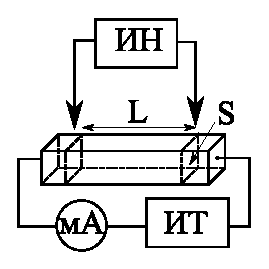
\includegraphics{pic1_1.eps}
\caption{Принципиальная схема двухзондового метода измерения удельного сопротивления: ИТ – источник тока; ИН – измеритель напряжения; $L$ – расстояние между зондами; $S$ – площадь сечения образца}
\label{1_base_scheme}
\end{figure}

Если по образцу протекает электрический ток силой $I$, создающий благодаря постоянству сечения образца одинаковую плотность тока в любой точке образца, то, измерив падение напряжения U между эквипотенциальными поверхностями, на которые установлены зонды, можно найти удельное сопротивление $\rho$ по формуле
\begin{equation}
\rho = \frac{U S}{I L}
\end{equation}

При этом предполагается, что эквипотенциальные поверхности перпендикулярны вектору плотности тока и сопротивлением контактов «зонд-полупроводник» можно пренебречь. Если первое условие при небольших сечениях образца удовлетворить легко, то второе условие, как правило, не удовлетворяется в силу особенностей контактных явлений между металлом и полупроводником.

Сопротивление образца на участке $x$ равно
\begin{equation}
R(x) = \int\limits_{0}^{x} {\frac{\rho(x)}{S} d x}
\end{equation}

Для однородного образца $\rho = const$ и $R(x) = \frac{d x}{S}$ - линейная функция от расстояния $x$. Если образец неоднороден, то зависимость $R(x)$ нелинейна, а сопротивление $\rho(x)$ можно найти по формулам

\begin{equation}
\begin{split}
\rho(x) &= S \cdot \tg(\phi) \\
\tg(\phi) &= \frac{d R}{d x} = \frac{\Delta R}{\Delta L}
\end{split}
\label{1_rho}
\end{equation}

\subsection{Анализ паразитных явлений и методика их устранения в двухзондовых измерениях удельного электросопротивления}

Пренебрежение влиянием контактных явлений может привести к грубым ошибкам измерения удельного сопротивления двухзондовым методом. Поэтому остановимся на описании вклада этих явлений подробнее.

\paragraph{Переходное сопротивление контакта «зонд-полупроводник».}
Из-за потенциального барьера (контактной разности потенциалов) вольтамперная характеристика (ВАХ) контакта металл-полупроводник является нелинейной, то есть сопротивление контакта зависит от величины и направления проходящего через него электрического тока. При измерении с помощью вольтметра падения напряжения между зондами в случае запирающих контактов, когда потенциальный барьер препятствует прохождению основных носителей заряда, один из контактов будет обладать высоким сопротивлением, которое может оказаться сопоставимым с внутренним сопротивлением вольтметра. Это внесет грубую ошибку в результат измерений. Избавиться от этой ошибки помогает компенсационный метод измерения падения напряжения, принципиальная схема которого представлена на рисунке \ref{1_potenc}. Для измерения падения напряжения используется потенциометр, представляющий собой калиброванный источник напряжения.

\begin{figure}[h!]\centering
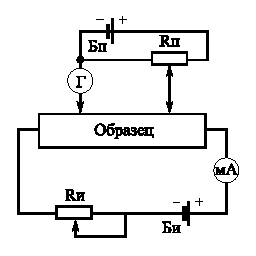
\includegraphics{pic1_2.eps}
\caption{Схема потенциометрического метода измерения}
\label{1_potenc}
\end{figure}

С помощью потенциометра $R_{\text{п}}$ между измерительными зондами создается компенсирующее напряжение $\text{Б}_{\text{п}}$, равное по величине и противоположное по знаку измеряемому. Последовательно с потенциометром в измерительную цепь включается чувствительный нуль-гальванометр Г. Если компенсирующее и измеряемое напряжение $\text{Б}_{\text{и}}$ равны по величине, то нуль-гальванометр фиксирует равенство нулю электрического тока, протекающего через измерительные зонды. В этом случае даже при высоком переходном сопротивлении контакта «зонд-полупроводник» падение напряжения на этом переходном сопротивлении равно нулю ($U_{\text{зонд}} = I R_{\text{зонд}} = 0$, т.к. $I = 0$).

Здесь следует добавить два важных замечания. Во-первых, внутреннее сопротивление потенциометра шунтирует сопротивление образца в цепи электрического тока, текущего через образец от источника тока, поэтом всегда должно соблюдаться требование $R_{\text{п}} \gg R_{\text{образца}}$. С учетом этого применяются для различных диапазонов измеряемых сопротивлений высокоомные потенциометры постоянного тока (ППТВ). Во-вторых, если нуль-гальванометр показывает равенство тока нулю, то это может означать, что протекающий ток меньше предела чувствительности гальванометра. Поэтому если использовать для измерения падения напряжения прибор, потребляющий электрический ток не выше предела чувствительности гальванометра, то он может заменить компенсационную схему измерения (то есть, обеспечить ту же погрешность измерения за счет вклада переходного сопротивления контактов).

\paragraph{Вклад паразитных термоЭДС.}

При измерении на высоких токах вдоль образца может возникать паразитная термоЭДС. Причиной появления термоЭДС является градиент температуры, возникающий при неравномерном разогреве образца за счёт протекающего тока. Знак этого градиента температуры не зависит от направления электрического тока. Благодаря этому такая термоЭДС может легко быть исключена из данных измерений при проведении двух измерений падения напряжения $U_{1}^{+}$ и $U_{2}^{-}$ между зондами при двух различных направлениях электрического тока. Падение напряжения на образце $U_{\text{обр}}$ и величину термоЭДС можно найти, определяя полусумму или полуразность величин $U_{1}^{+}$ и $U_{2}^{-}$ с учётом их знака.

\begin{equation}
\begin{split}
U_{1}^{+} &= I R_{\text{обр}} + U_{\text{ТЭДС}} \\
U_{2}^{-} &= -I R_{\text{обр}} + U_{\text{ТЭДС}} \\
U_{\text{обр}} &= I R_{\text{обр}} = \frac{U_{1}^{+} - U_{2}^{-}}{2} \\
U_{\text{ТЭДС}} &= \frac{U_{1}^{+} + U_{2}^{-}}{2}
\end{split}
\label{Uteds}
\end{equation}

Если токовые контакты не являются омическими, то при прохождении тока в них может возникать эффект Пельтье, то есть нагревание или охлаждение контакта в зависимости от направления тока. ТермоЭДС, создавшуюся в результате такого градиента температуры, вышеописанным способом устранить невозможно, так как она будет изменять знак с изменением направления тока. Неомичность токовых контактов также может привести к возникновению взаимосвязанных явлений инжекции, эксклюзии, экстракции и аккумуляции в приконтактных областях образца, которые могут изменить истинную величину электросопротивления. Следует делать минимальной величину тока, протекающего в образце, чтобы избежать разогрева образца, а также защищать образец от освещения во избежание возникновения в нем фотопроводимости или контактных фотоэдс. Все эти явления могут давать существенную погрешность измерения в высокоомных образцах.

\section{Описание измерительной установки}

Принципиальная электрическая схема установки показана на рисунке \ref{1_scheme}

\begin{figure}[h!]\centering
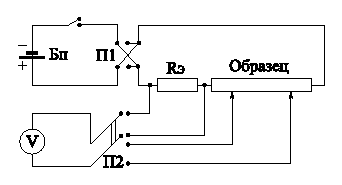
\includegraphics{pic1_3.eps}
\caption{Принципиальная схема измерений двухзондовым методом}
\label{1_scheme}
\end{figure}

Величина электрического тока через образец устанавливается при помощи управляемого линейного источника питания Б5-30. Точное определение тока производится по измерению падения напряжения $V$ на эталонном сопротивлении $R_{\text{э}}$, включённом последовательно с сопротивлением образца $R_{\text{обр}}$. Переключатель П2 может подключать вольтметр В7-21А или к образцу, или к эталонному сопротивлению. Переключатель П1 меняет направление электрического тока в образце. Источник тока может быть заменён батареей с подключённым последовательно переменным сопротивлением.

Исследуемый образец с нанесенным омическими контактами помещается в токовые зажимы на предметном столе в поле зрения оптического микроскопа. Определение расстояния между измерительными зондами производится с помощью микрометрической головки микроскопа. Нулевое положение устанавливается при совмещении перекрестия в поле зрения микроскопа с изображениями соприкасающихся первого и второго зондовых контактов. Полный оборот микрометрической головки микроскопа соответствует перемещению перекрестия на 1 мм.

Для определения типа проводимости образца применяется метод термозонда, принципиальная схема которого изображена на рисунке \ref{1_condtype}. Образец помещается на массивную металлическую пластину, служащую «холодным» контактом. Вместо массивного основания можно использовать холодный щуп. Нагретым с помощью небольшого электронагревателя зондом касаются верхней поверхности образца. Если образце имеет место проводимость n-типа, то электроны в образце диффундируют от нагреваемой термозондом верхней грани к «холодной» нижней грани, заряжая ее отрицательно. Верхняя грань образца будет заряжаться положительно за счет остающихся нескомпенсированными ионов донорной примеси $N_{D}^{+}$. Если образец имеет p-тип проводимости, то к «холодной» грани образца диффундируют положительно заряженные дырки, оставляя на «горячей» грани отрицательный заряд $N_{A}^{-}$ нескомпенсированных ионов акцепторов. Если в качестве регистрирующего устройства между горячим и холодным зондом включить параллельно светодиоды разного цвета, то при изменении типа проводимости измениться направление тока в цепи диодов и включится тот, напряжение на котором будет прямым. В используемом в работе детекторе в образце n-типа проводимости загорается зеленый светодиод, в образце p-типа — красный.

\begin{figure}[h!]\centering
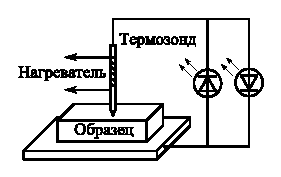
\includegraphics{pic1_4.eps}
\caption{Принципиальная схема измерений двухзондовым методом}
\label{1_condtype}
\end{figure}

\section{Порядок проведения работы и указания по технике безопасности}

\begin{enumerate}
\item Измерить толщину и ширину образца.
\item Установить образец на предметном столике и опустить на его поверхность измерительные зонды достаточно далеко от токовых контактов.
\item Установить необходимую величину тока через образец.
\item Привести в соприкосновение оба зонда, отметить нулевую точку отсчета на микрометрической головке микроскопа.
\item Повернуть микрометрическую головку микроскопа на 360\textdegree, переместить подвижный зонд на 1 мм по поверхности образца (конец зонда должен совместиться с перекрестьем в поле зрения микроскопа).
\item Измерить величину $U_{1}^{+}$ и $U_{2}^{–}$ с освещением и без освещения образца. Занести данные в таблицу \ref{1_table}.
\item Повторить п.п. 5 и 6.
\item Рассчитать зависимость $U_{\text{обр}}$ от расстояния $L$.
\item Изменить величину тока через образец и повторить измерение $U_{\text{обр}}$ от расстояния $L$.
\end{enumerate}

Электрический ток в измерительной схеме не превышает 3мА.

\section{Обработка результатов эксперимента}

\begin{enumerate}
\item Результаты измерений занести в таблицу \ref{1_table}, отметив условие освещённости образца.
\item Построить графики $R_{\text{обр}} = f(L)$ и $U_{\text{ТЭДС}} = f(L)$.
\item В соответствии с формулами (\ref{1_rho}) рассчитать $\rho(x)$.
\item Построить график $\rho(L)$ и сопоставить его с графиком $U_{\text{ТЭДС}}(L)$. Выполнить это построение для различных значений тока через образец и условий его освещенности.
\item Рассчитать погрешность измерения сопротивления Rобр и l и нанести их на графики.
\item Оценить погрешность определения удельного сопротивления $\delta \rho$.
\item Высказать суждение об однородности или неоднородности образца и влиянии величины электрического тока через образец и условий его освещенности на результаты измерений.
\end{enumerate}

\begin{table}[h]
\renewcommand{\arraystretch}{1.8} %% increase table row spacing
\caption{Измерение удельного электросопротивления при освещении (без освещения)}
\begin{center}
\begin{tabular}{c|c|c|c|c|c|c|c|c}
№ & $L$ & $U_{\text{э}}$ & $I = \frac{U_{\text{э}}}{R_{\text{э}}}$ & $U_{1}^{+}$ & $U_{2}^{-}$ & $U_{\text{обр}}$ & $U_{\text{ТЭДС}}$ & $R_{\text{обр}}$ \\
\hline
& мм & мВ & мА & мВ & мВ & мВ & мВ & Ом \\
\hline
\end{tabular}
\end{center}
\label{1_table}
\end{table}

\section{Контрольные вопросы}
\begin{enumerate}
\item Почему для определения удельной электропроводности полупроводниковых материалов применяют зондовые методы?
\item Достоинства и недостатки двухзондового метода измерения удельной электропроводности полупроводниковых материалов.
\item Как определить удельное сопротивление однородного и неоднородного образца при измерении двухзондовым методом?
\item Механизмы электропроводности в полупроводниках и металлах.
\item Какими факторами определяется величина концентрации свободных носителей заряда в полупроводниках и металлах при комнатной температуре?
\item Чем определяется температурная зависимость электропроводности полупроводников и металлов?
\item Какие процессы определяют появление свободных носителей заряда в области собственной и примесной проводимости?
\item От каких факторов зависит температура перехода от примесной проводимости к собственной?
\item Какие примеси создают n- или p- проводимость в полупроводнике?
\item Как влияет освещение на электропроводность полупроводников?
\item Какие материалы при измерении электропроводности необходимо затенять и почему?
\item Понятие механизма рассеяния свободных носителей заряда.
\item Назовите основные механизмы рассеяния свободных носителей заряда в полупроводниках и металлах.
\item В чем проявляется отличие свойств свободного электронного газа полупроводников и металлов?
\item Как влияет кристаллическое совершенство материала на электропроводность полупроводников и металлов?
\end{enumerate}

\section{Литература}
\begin{enumerate}
\item К.В. Шалимова. Физика полупроводников. СПб.: Лань, 2011 г.
\item В.В. Батавин, Ю.А. Концевой, Ю.В. Федорович. Измерение параметров полупроводниковых материалов и структур. М.: Радио и связь, 1985 г.
\item Л.П. Павлов. Методы определения основных параметров полупроводниковых материалов. М.: Высшая школа, 1975 г.
\item В.В. Горбачев, Л.Г. Спицина. Физика полупроводников и металлов. М.: Высшая школа, гл. 1, 1986 г.
\end{enumerate}
\newpage

\anonchapter{������������ ������ �2}
\setcounter{chapter}{2}

\begin{center}
����������� ������ ����������� ���� �������������� \\
(4 ����)
\end{center}

\section{���� ������}
����������� ������ ����������� ���� � �������-���������� ������ �� ������ ��������� ������������� ����������� ������������������.

\section{������������� �����}
\subsection{������������� ����������� ������������������}

����������� ���������, ���������� ������������� �� �������, �������� ���������� ������������������ ��������������� ��� ��������� �����������.

��� �������������� � ����� ���������� ����� ������������ �������� ������������������ ����� ����������� � ����:
\begin{equation}
\sigma = e n \mu
\end{equation}
��� $e$ - ����� ���������, $n$ - ������������ �������, $\mu$ - ����������� ��������� ������.

��� ������������ ������������������ � ������� � ������ ������ ���������, ���������� ��������� ������ ������� �� ���:
\begin{equation}
\sigma = e n \mu_{n} + e p \mu_{p}
\end{equation}

��� ������� ������������� ����������� �������������� ���������� ������� ����������� �� ����������� � ������������ ��������� ��������� ������ (���).

\subsection{������������� ����������� ����������� ���}

��� ������� ���������� ��������� ������������� n-����. �� ������� \ref{pic2_zone} �������� �������������� ��������� ��������� ��������������. ����� ��� ����������� ������������ �� ����������� ��� �������������� �������������� � ����� ����� �������� ������� ����������� �� ������� \ref{pic2_n_T}.

\begin{figure}[h!]\centering
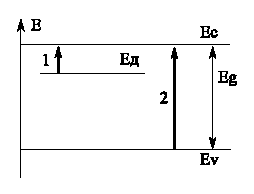
\includegraphics[height=4cm]{pic2_zone.eps}
\caption{������ ��������� � ����� ����� �������� �������}
\label{pic2_zone}
\end{figure}

\begin{figure}[h!]\centering
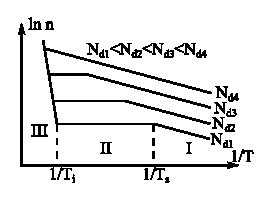
\includegraphics[height=4cm]{pic2_n_T.eps}
\caption{����� ��� ������������� ����������� ������������ ��� �������������� �������������� � ����� ����� �������}
\label{pic2_n_T}
\end{figure}

�� ����������� $\ln n = f(\frac{1}{T})$ ����� �������� ��� ����������� ������������� ���������.

\paragraph{I. ������� ��������� ���������.}
��� ���������� ���� ��������� ���� �������������� ������� ��������� �����������. � ���� ������������ ��� ��������� ���������. ��� ��������� ����������� ��������� ��������� � ������� �������� ������� � ���� ������������, ������������ ��������� ���������� ����������. ��� ������� ���������� ���������� ������ ������� � ������������ ������ �� ����������� ��������� ������� $T = T_{s}$. � ���� �������
\begin{equation}
n = \sqrt{\frac{N_{c}N_{d}}{2}} \exp{\left( -\frac{E_{d}}{2 k T} \right)}
\label{eq2_n_T}
\end{equation}
��� $N_{c} = 2 \left( \frac{2 \pi m_{dn}^{*} k T}{h^2} \right) ^ \frac{3}{2}$ - ����������� ��������� ��������� � ���� ������������, $E_{d}$ - ������� ��������� �������� �������, $N_{d}$ - ������������ �������.

\paragraph{II. ������� ��������� �������.}
� ������� ���������� $T_{s} < T < T_{i}$ �������� ������� ��������� ����������, �� ����������� ��������� ��� �� ��������. ������� ������������ ��������� ���������� ��������� � ����� $N_{d}$.
������ ������� ��������� ������� �� ������������ ������������ ������� � � ������� ���������. ��� ���������� ���� ������� ������������� �������� ������� ��������� ����� �����������. ��� ���������� ������� ��������� $N_{d}$ �� ����� ��������� ���������.

\paragraph{III. ������� ����������� ���������.}
� ������� ������� ���������� $(T > T_{i})$, ����� ������� ��������� �������� ���������� ���������� ������������ � ������� ����������� ���� $(k T \approx E_{g})$, ��������� �������� ���������� �� ��������� ���� � ���� ������������, ��-�� ���� ������������ ��������� ��������� ����� ����������. ���������� ��������� ������ ��������� �������.

\begin{equation}
n_{i} = \sqrt{N_{c} N_{v}} \exp{\left( -\frac{E_{g}}{k T} \right)} \sim T^{\frac{3}{2}} \exp{\left( -\frac{E_{g}}{k T} \right)}
\label{eq2_ni_T}
\end{equation}

������ ����������� ���� ����� ������� �� �����������. ��� ����������� ��������������� �������� $E_{g}$ ������� ������� ��������� � ������������, ������ � ������� ��������� ���������� ��� ����� ���� ���������������� ������ ������:
\begin{equation}
E_{g}(T) = E_{g}(0) + \alpha T
\label{eq2_E_T}
\end{equation}
��� $E_{g}(0)$ - ��������, ������� ����� �������� �������������� ������������� ����������� ������ ����������� ���� �� �������� 0\textdegree �, $\alpha$ - ������������� ����������� ��������� ������ ����������� ����, ������ ����������� � ���������� ������� ���� ���/�.

�� ������� \ref{pic2_E_T} �������� ������������� ����������� ������ ����������� ���� � �������.

\begin{figure}[h!]\centering
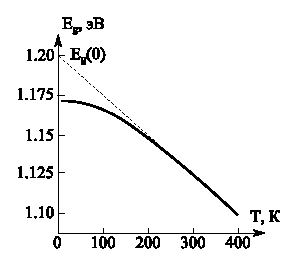
\includegraphics[height=4cm]{pic2_E_T.eps}
\caption{������������� ����������� ������ ����������� ���� ��� �������}
\label{pic2_E_T}
\end{figure}

���������� (\ref{eq2_E_T}) � (\ref{eq2_ni_T}) ��������:
\begin{equation}
n_{i} = \sqrt{N_{c} N_{v}} \exp{\left( -\frac{E_{g}(0) + \alpha T}{k T} \right)} \sim T^{\frac{3}{2}} \exp{\left( -\frac{E_{g}(0)}{k T} \right)} \exp{\left( -\frac{\alpha}{k} \right)}
\label{eq2_ni_T}
\end{equation}

\subsection{������������� ����������� ����������� ���}
����������� ����� ������� �� �����������. �������� ����������� ������������ ������������ ���������� ��������� � �������������� ��� ������ �����������. ��� ����������� ���������� ����������� $\mu(T)$ ����� ���� ���������� ��������� �����������:
\begin{equation}
\mu(T) = \mu_{i} \left( \frac{T}{T_{i}} \right)^{m}
\end{equation}
��� $\mu_{i}$ - ����������� ��� ����������� $T = T_{i}$.

���� �������� ���������� �������� ��������� �� ����� �������, ���������� $m = \frac{3}{2}$. ��� ��������� �� ����������� �������� $m = 0$, � ��� ��������� �� ������������ ������� $m = -\frac{3}{2}$. � �������� ��������������� ������������ ��������� ��������� ���������� ���������, ������� ����������� �������� ���������� $m$ ����� ��������� ������ ��� ������������� ��������� ����������. ��� ���� ��������� ���������� ��������� - �� ������������ ������� � ����� ������� - ������������� ���������� ����������� ��������� ���, ���������� �� ������� \ref{pic2_mu_T}

\begin{figure}[h!]\centering
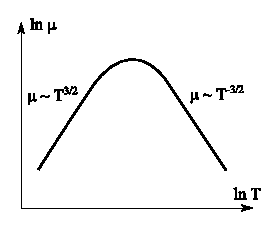
\includegraphics[height=4cm]{pic2_mu_T.eps}
\caption{������������� ����������� ����������� ��������� ��������� ������ � ������������� ��������������}
\label{pic2_mu_T}
\end{figure}

� ������� ������ ���������� ������������ ���������� ��������� �������� ��������� �� ����� �������. � ������ ����������� ����������� �������������, ��� ��� ������������� �������� �������� ���������, � ��� �������������� � ������������� �������� (��������� ������) �������� ����������� �� ������� ����. � ���������� ������ ����������� ������� ���������� ��������� �������� ��������� ������� �������, � ����������� �������������� ���������� �� ������������ �������, �������. ��� ���� ����� � �������� ��������������� ���������� ����������� ��� ������ ������ ����� ���������� �� ���������� �������� $m = -\frac{3}{2}$ � ������� ���� � �� ��� ������ �������.

� ������ ������ (\ref{eq2_n_T}) � (\ref{eq2_ni_T}) ����� ��������� ����������� ������������������ �� �����������. ��������� ��� ����� ����������� ������� �� ������� \ref{pic2_sigma_T}.

\begin{figure}[h!]\centering
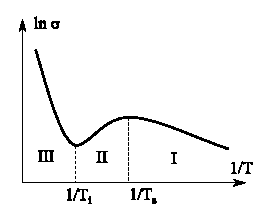
\includegraphics[height=4cm]{pic2_sigma_T.eps}
\caption{������������� ����������� ������������������ � ������������� ��������������}
\label{pic2_sigma_T}
\end{figure}

�� ���������� ������� ����� �������� ��� �������.

I. ������� ��������� ������������
\begin{equation}
\sigma = e n(T) \mu(T) \sim T^{\frac{3}{4} + m} \exp{\left( -\frac{E_{d}}{2 k T} \right)}
\end{equation}

II. ������� ��������� �������
\begin{equation}
\sigma = e N_{d} \mu(T) \sim N^{m}
\end{equation}

III. ������� ����������� ������������
\begin{equation}
\sigma_{i} = e n_{i}(T) \left[ \mu_{n}(T) + \mu_{p}(T) \right] \sim T^{\frac{3}{2} + m} \exp{\left( -\frac{\alpha}{2 k} \right)} \exp{\left( -\frac{E_{g}(0)}{2 k T} \right)}
\end{equation}

� ���������� ����������� ���� ��������� ����������� ������������. � ������� ��������� ������� ������������� ����������� ������������������ ������������ ������������� ������������ �����������. � �������� ��������� � ����������� ��������� ������� ������� ��������� ������������� ����������� ������������ ���������.

���� ���������� ������ ��������� ����������� ������ ����������� ���� �� �����������, �� ������� (I) � (III) ����� ��� ������ � ��������� ���� ������� $-\frac{E_{d}}{2 k T}$ � $-\frac{E_{g}(0)}{2 k T}$ ��������������. ����� �������, ����������������� ����������� ��������� ������������ �� �������� ����������� ��������� ���������� ������� ��������� � ������ ����������� ���� �����������������. ��� ���� ����� �������, ��� �������� $E_{g}(0)$ �� ����� � �������� ������ ����������� ���� � �������������� ��� ����������� 0\textdegree �, � �������� ������, � ������� �������� ������������� ����������� ��� ������� ���������� ���������� ��� �������. ������ ��� ����������� $E_{g}$ �� ����� ������������� ����� ��������� ������ ���������.

\section{�������� ��������� � �������� ���������}

� ������ ������ ������������ �����, ���������� �� ������� \ref{pic2_scheme}. ������� $R_{\text{���}}$ ���������� � ���� ��������������� � �������� - ������� �������������� ������� ��������� �������� $R_{\text{���}}$. � ���� ��������� ����� ���� ������������ ���, ��� ���� ������� ���������� �� $R_{\text{���}}$ � $R_{\text{���}}$ ��������� ��� ������ �������������� ������ Fractal MCX 52.1. �������� ���� ����� ������� $I_{\text{���}}$ ����� ���� ����� ��������� ������������� � ����� ���� ������� ���
\begin{equation}
I_{\text{���}} = I_{\text{���}} = \frac{U_{\text{���}}}{R_{\text{���}}}
\end{equation}

\begin{figure}[h!]\centering
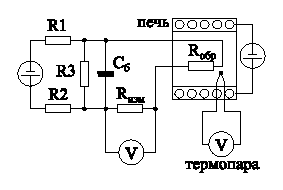
\includegraphics[height=4cm]{pic2_scheme.eps}
\caption{�������������� ����� ��������� ��� ��������� ������������� ����������� ��������������������}
\label{pic2_scheme}
\end{figure}

��� ��� ���������� ���������������� �����-������ ��� � ������� ������ MCX ��������� � ��������� �� $0.02$ �� $2.56$ �, �� � ����� ������������ �������� ����������, ����������� �� ���������� $R1$, $R2$ � $R3$.

����� ��������� ������� ��������, ������� ����� ���������� ��-�� ��������� ����������� ����� �������, ��������� ������������ ��������� ���������� � ���� ������������. ����������� $C_{\text{�}}$ ���������� ����������� ���������, �������� ������� ����.

������� � ����������� ��������� ���������� � ��������� ������ �����������, ������� �������� �������������� �� ��������� �378. ����������� ������� ���������� ����������, ������ � ������� ������������� ��������������� ������������� ������� MCX 52. ���������� ��������� ������� ���������� �� �������, ��������� ������������� � ������ � ��������� ��������������� ���������� ��� � ���������� �� ���������, ��� �� ���������� � ������ ���������� � ������������� ������ ��������������� � ������������� ����������� ������� � �����������.

\section{������� ���������� ������ � �������� �� ������� ������������}

\begin{enumerate}
\item ��������� ��������� ��� ��������� ������������� ����������� ��������������������.
\item ���������� ����� <<���������>> � ������� ������������ � ������ ������ COM-port.
\item ��������� ��������� � �������� ������, ����� 50� �� �����������.
\item ������� ������� �� 120\textdegree C.
\item ��������� ������, �������� ������� �� 40\textdegree C.
\item ��������� ���������� ���������.
\end{enumerate}

����� ������� ��������� ���������� ��������� � ���, ��� �������� ����� � �������� ��������� ���������. ��� ������ � ����� ����������� ��������� ����������� ���� 200\textdegree C.

\section{��������� ����������� ������������}

\begin{enumerate}
\item ���������� ��������� ������� � �������, ������� ������� ������� � ����������.
\item ���������� �������� ��������� � ����������� $\ln \sigma = f \left( \frac{1}{T} \right)$.
\item �� ���������� ������� (��������� ��� ������� �� ������� \ref{pic2_experiment}) �������� ��� �������� �������, ����� ������������� ����������� ������������, ������ - ���������.
\item ������ ������ ������������ ��������� ������� ���������. � ������� ����������� ������������ $\tg (\phi_{2}) = -\frac{E_{g}(0)}{2 k}$, ������ $E_{g}(0) = -2 k \tg(\phi_{2})$.
\item ���������� ���������� ������� ��������� ������� $E_{d} = -2 k \tg(\phi_{1})$.\
\item ���������� ������ ���������, ��������� ������� ��������� �� ��������� �������� ������.
\end{enumerate}

\begin{table}[h!]
\caption{��������� ��������� �������������������� ��� ��������� (��� ���������)}
\begin{center}
\begin{tabular}{c|c|c|c|c|c|c|c}
� & $U$ & $t$ & $T$ & $R$ & $\sigma$ & $\ln(\sigma)$ & $\frac{1}{T}$ \\
\hline
& �� & \textdegree C & � & �� & $\text{��}^{-1} \text{��}^{-1}$ &  & K \\
\hline
\end{tabular}
\end{center}
\end{table}

\begin{figure}[h!]\centering
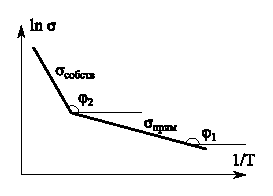
\includegraphics[height=4cm]{pic2_experiment.eps}
\caption{�������� ��� ������������� ����������� ������������������ ��������������}
\label{pic2_experiment}
\end{figure}

\section{����������� �������}

\begin{enumerate}
\item ������� ������ ����������� ���� � ������� ��������� �������.
\item ������������� ����������� ������ ����������� ���� � ���������������.
\item ������������� ����������� ������������ ��������� ��� �������������� �������������� � ���� ���������� ����� ������������.
\item ��������� ��������� ��������� ������ � ���������������.
\item ������������� ����������� ����������� ��������� ����� � ���������������.
\item ������������� ����������� ������������������ � ���������������.
\item ����������� ������� ��������� ������� �� ������������� ����������� ��������������������.
\item �������� �������, ������������� �������� ���������.
\end{enumerate}

\section{����������}

\begin{enumerate}
\item �.�. ������. ����� ��������������. �.: ������ �����, 1975.
\item �.�. ��������, �.�. �������. ������ ��������������� � ��������. �.: ������ �����, ��. 3, 1986 �.
\item �.�. ������. ������ ����������� �������� ���������� ����������������� ����������. �.: ������ �����, 1975 �.
\end{enumerate}
\newpage

\anonchapter{Лабораторная работа №3}
\setcounter{chapter}{3}
\setcounter{section}{0}
\setcounter{figure}{0}
\setcounter{table}{0}
\setcounter{equation}{0}

\begin{center}
Определение подвижности основных носителей заряда \\
(4 часа)
\end{center}

\section{Цель работы}
Определение подвижности основных носителей заряда в полупроводнике и коэффициента Холла по измерениям эффекта холла.

\section{Теоретическая часть}

\subsection{Возникновение поля Холла}

Эффект Холла заключается в возникновении поперечного электрического поля в образце, через который протекает электрический ток, помещённом в магнитное поле, перпендикулярное направлению этого тока. Если в магнитном поле с индукцией $\overrightarrow{B}$ находится полупроводник n-типа, по которому течёт ток плотностью $\overrightarrow{j}$, то на электроны, движущиеся со скоростью $\overrightarrow{v}$ будет действовать сила Лоренца, отклоняющая их в сторону. Таким образом, на одной из граней появится отрицательный заряд, а на другом начнут скапливаться нескомпенсированные доноры. В дырочном полупроводнике механизм останется тем же, но знаки зарядов и направление их движения изменятся (см. рисунок \ref{pic3_lorentz}).

\begin{figure}[h!]\centering
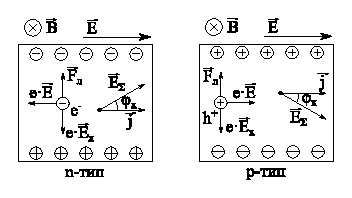
\includegraphics[height=4cm]{pic3_lorentz.eps}
\caption{Проявление эффекта Холла в образцах n- и p-типа проводимости.}
\label{pic3_lorentz}
\end{figure}

Возникающие на гранях, параллельных течению тока и индукции магнитного поля, заряды, создают электрическое поле $\overrightarrow{E}_{\text{х}}$, стремящееся компенсировать отклонение зарядов под действием силы Лоренца. Суммарное поле $\overrightarrow{E}_{\Sigma}$ будет направлено под углом $\phi$ к току, направление которого не изменится. Напряжённость поля $\overrightarrow{E}_{\text{х}}$ пропорциональна векторному произведению $\overrightarrow{B}$ и $\overrightarrow{j}$ с коэффициентом пропорциональности $R_{\text{х}}$.

\begin{equation}
\overrightarrow{E}_{\text{х}} = \overrightarrow{R}_{\text{х}} \left[ \overrightarrow{B} \times \overrightarrow{j} \right]
\label{eq3_vector_lorentz}
\end{equation}

$R_{\text{х}}$ называется коэффииентом Холла, а $\phi$ - углом Холла.

Как видно из рисунка \ref{pic3_lorentz}, направление силы Лоренца не зависит от знака заряда, а значит по направлению поля Холла можно определить тип основных носителей заряда в полупроводнике. Коэффициент Холла отрицателен в полупроводнике n-типа, и положителен для p-типа.

\subsection{Определение коэффициента Холла}

Если все углы между $\overrightarrow{B}$, $\overrightarrow{j}$ и $\overrightarrow{E}_{\text{х}}$ прямые, и не учитывается распределение электронов по скоростям, то (\ref{eq3_vector_lorentz}) можно переписать как

\begin{equation}
E^{y}_{\text{х}} = \frac{1}{e n} j^{x} B^{z}
\end{equation}
где $e$ - заряд электрона, $n$ - концентрация свободных носителей заряда.

В таком случае $R_{\text{х}} = \frac{1}{e n}$. Для учёта различия между полной скоростью электронов, входящей в выражение для силы Лоренца, и дрейфовой скоростью, которую электрон принимает под действием поля, а также распределения электронов по скоростям, решается кинетическое уравнение Больцмана. Точное решение приводит к необходимости введения коэффициента $r_{\text{х}} = \frac{<\tau^{2}>}{<\tau>^2}$, называемого холл-фактором, $\tau$ - время релаксации при данном основном механизме рассеяния.. В таком случае полное выражение для коэффициента Холла выглядит следующим образом:

\begin{equation}
R_{\text{х}} = \frac{r_{\text{х}}}{e n}
\end{equation}

Расчёты показывают, что для невырожденных полупроводников при рассеянии на акустических фононах $r_{\text{х}} = \frac{3}{8} \pi$, а при рассеянии на ионах примеси $r_{\text{х}} = \frac{315}{512} \pi$. Для вырожденных полупроводников и металлов величина $r_{\text{х}}$ от доминирующего механизма рассеяния не зависит и равна единице. Для сильных магнитных полей ($\mu B \gg 1$) коэффициент Холла не зависит от механизма рассеяния и степени вырождения, а определяется только концентрацией носителей заряда: $R_{\text{х}} = \frac{1}{e n}$.

В случае смешанной проводимости и в материалах близких к собственным коэффициент Холла опреедляется следующим соотношением:
\begin{equation}
R_{\text{х}} = \frac{r_{\text{х}}}{e} \frac{p \mu_{p}^{2} - n \mu_{n}^{2}}{\left( p \mu_{p} + n \mu_{n} \right)^{2}}
\end{equation}

В области примесной проводимости по коэффициенту Холла и электропроводности можно определить концентрацию основных носителей заряда, а по тангенсу угла Холла - их подвижность.

\subsection{Методика измерения и описание установки}

В ходе данной работы через образец, имеющий форму прямоугольного параллелепипеда, пропускается постоянный ток, и измеряется разность потенциалов, возникающая на холловских контактах (см. рисунок \ref{pic3_sample}). В данном случае

\begin{equation}
\begin{split}
V_{\text{х}} &= b E_{\text{х}} \\
V &= a E \\
I &= b d j
\end{split}
\end{equation}

\begin{figure}[h!]\centering
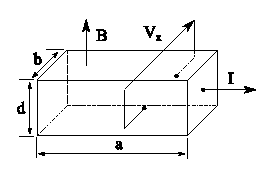
\includegraphics[height=4cm]{pic3_sample.eps}
\caption{Линейные размеры образца и расположение основных векторов}
\label{pic3_sample}
\end{figure}

Эти формулы можно переписать в виде:
\begin{equation}
\begin{split}
V_{\text{х}} &= - \frac{R_{\text{х}} I B}{d} \\
V &= \frac{I}{\sigma} \frac{c}{b d}
\end{split}
\end{equation}

Угол между направлением электрического поля в образце и полем Холла называется углом Холла и определяется как:
\begin{equation}
\tg \phi = \frac{E_{\text{х}}}{E} = \frac{a}{b} \frac{V_{\text{х}}}{V}
\label{eq3_tg}
\end{equation}

Измерив падение напряжения в продольном и поперечном направлении, а также индукцию магнитного поля, можно рассчитать основные характеристики образца:
\begin{equation}
\begin{split}
\sigma &= \frac{c}{b d} \frac{I}{V} \\
R_{\text{х}} &= d \frac{V_{\text{х}}}{I} \frac{1}{B} \\
\mu_{\text{х}} &= \frac{c}{b} \frac{V_{\text{х}}}{V} \frac{1}{B}
\end{split}
\label{eq3_mu}
\end{equation}

На точность измерения эффекта Холла влияет геометрия образца. Поперечное напряжение можно считать равным ЭДС Холла только при отношении длины образца к ширине не менее $3:1$.

Для измерения коэффициента Холла применяется стандартный метод постоянного тока и постоянного магнитного поля. Уменьшение вклада паразитных эффектов производится усреднением результатов измерения при разных направлениях тока и индукции. Пусть

\begin{equation}
\begin{split}
V_{I^{+}B^{+}} &= V_{\text{х}} + V_{\text{асм}} + V_{\text{мр}} + V_{\text{ТЭДС}} + V_{\text{Э}} + V_{\text{НЭ}} + V_{\text{ПНЭ}} + V_{\text{РЛ}} + V_{\text{ПРЛ}} \\
V_{I^{-}B^{+}} &= -V_{\text{х}} - V_{\text{асм}} - V_{\text{мр}} + V_{\text{ТЭДС}} - V_{\text{Э}} + V_{\text{НЭ}} - V_{\text{ПНЭ}} + V_{\text{РЛ}} - V_{\text{ПРЛ}} \\
V_{I^{-}B^{-}} &= V_{\text{х}} - V_{\text{асм}} - V_{\text{мр}} + V_{\text{ТЭДС}} + V_{\text{Э}} - V_{\text{НЭ}} + V_{\text{ПНЭ}} - V_{\text{РЛ}} + V_{\text{ПРЛ}} \\
V_{I^{+}B^{-}} &= -V_{\text{х}} + V_{\text{асм}} + V_{\text{мр}} + V_{\text{ТЭДС}} - V_{\text{Э}} - V_{\text{НЭ}} - V_{\text{ПНЭ}} - V_{\text{РЛ}} - V_{\text{ПРЛ}}
\end{split}
\end{equation}

$V_{\text{х}}$ - напряжение Холла.

$V_{\text{асм}}$ - напряжение асимметрии, возникающее, если холловские контакты находятся не на эквипотенциальных поверхностях. Знак не зависит от направления магнитного поля, но меняется вместе с направлением электрического поля.

$V_{\text{мр}}$ - магниторезистивный эффект, меняющий напряжение асимметрии. Знак зависит от направления тока.

$V_{\text{ТЭДС}}$ - термоэлектрический эффект, возникает между контактами при наличии градиента температур, одним из источников которого может быть неравномерность нагрева неоднородного образца. Зависит только от знака градиента температуры.

$V_{\text{Э}}$ - поперечный гальвано-термомагнитный эффект Эттинсгаузена, возникающий из-за наличия определённого распределения носителей по скоростям. Под действием магнитного поля быстрые горячие электроны отклоняются сильнее медленных холодных, из-за чего возникает поперечный градиеннт температур и связанная с ними термоЭДС. Знак зависит от направления тока, направления магнитного поля и знака носителей заряда.

$V_{\text{НЭ}}$ - поперечный термогальваномагнитный эффект Нернста-Эттинсгаузена, возникает из-за наличия продольного градиента температур. Энергия электронов, движущихся от горячего конца к холодному больше энергии в обратном потоке, эти потоки отклоняются в магнитном поле в разные стороны, возникает ток в поперечном направлении, который компенсируется током за счет ЭДС Нернста-Эттинсгаузена. Знак зависит от направления магнитного поля.

$V_{\text{ПНЭ}}$ - электротермически эффект Пельтье, приводящий к термогальваномагнитному эффекту Нернста-Эттинсгаузена, наблюдается если причиной возникновения грандиента температур является эффект Пельтье вблизи омических контактов. Знак зависит от направления тока и магнитного поля.

$V_{\text{РЛ}}$ - термомагнитный эффект Риги-Ледюка, поперечная термоЭДС, возникающая из-за продольного градиента температур. Знак зависит от направления магнитного поля.

$V_{\text{ПРЛ}}$ - эффект Пельтье, приводящий к возникновению продольного градиент температур и, как следствие, к термоЭДС Риги-Ледюка. Знак зависит от направления тока и направления магнитного поля.

Усреднённое напряжение на холовских контактах рассчитывается по формуле:
\begin{equation}
\overline{V}_{\text{х}} = \frac{V_{I^{+}B^{+}} - V_{I^{-}B^{+}} + V_{I^{-}B^{-}} - V_{I^{+}B^{-}}}{4} = V_{\text{х}} + V_{\text{Э}} + V_{\text{ПНЭ}} + V_{\text{ПРЛ}}
\end{equation}

Вкладом эффектов Пельтье-нернста-Эттинсгаузена и Пельтье-Риги-Ледюка во многих материалах, особенно высокоомных, можно пренебречь.

Если оборудование позволяет изменять только направление магнитного поля, среднюю величину рассчитывают по разности измеренных значений при разной полярности магнитного поля:

\begin{equation}
\overline{V}_{\text{х}} = \frac{V_{I^{+}B^{+}} - V_{I^{+}B^{-}}}{2} = V_{\text{х}} + V_{\text{Э}} + V_{\text{НЭ}} + V_{\text{ПНЭ}} + V_{\text{РЛ}} + V_{\text{ПРЛ}}
\end{equation}

В ходе работы через образец, помещённый между полюсами магнита, пропускается ток и снимается разность потенциалов между токовыми и холловскими выводами. Полученные данные считываются встроенными в лабораторный стенд АЦП и обрабатываются микроконтроллером, после чего передаются на компьютер. Значение магнитной индукции в диапазонах, используемых в данной работе, линейно зависит от тока через катушку. Блок-схема прибора приведена на рисунке \ref{pic3_scheme}. Все указанные на схеме вольтметры встроены в лабораторный стенд и отображаются в рабочей области программы. Приборы активируются щелчком мыши по соответствующему значку.

\begin{figure}[h!]\centering
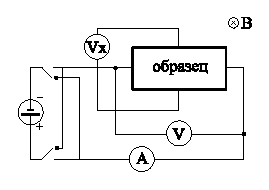
\includegraphics[height=4cm]{pic3_scheme.eps}
\caption{Линейные размеры образца и расположение основных векторов}
\label{pic3_scheme}
\end{figure}

\section{Порядок проведения работы и указания по технике безопасности}

\begin{enumerate}
\item Запустить прибор и программу для измерения эффекта Холла.
\item Выбрать схему измерения №1, активировать все блоки устройства.
\item Установить значение тока через образец равным 1 мА.
\item Провести серию измерений напряжения на образце $V$ и напряжения Холла $V_{\text{х}}$ изменяя индукцию магнитного поля от -150 до 150 мТл.
\item Повторить измерения при токе через образец равном 2 мА.
\end{enumerate}

Электрический ток в схеме не превышает 10 мА. При выполении работы действует стандартная техника безопасности при работе с компьютером.

\section{Обработка результатов эксперимента}

\begin{enumerate}
\item Результаты измерений занести в таблицу. Значения для положительных и отрицательных величин индукции магнитного поля вносятся в одну строку с указанием полярности.
\item Определить тангенс угла Холла из соотношения (\ref{eq3_tg}).
\item Определить тип и подвижность основных носителей заряда, пользуясь выражением (\ref{eq3_mu}).
\item Используя (\ref{eq3_mu}) найти коэффициент Холла, считая основным механизмом рассеяние на ионах примеси.
\item Определить погрешность измерения.
\end{enumerate}

\begin{table}[h!]
\caption{Измерение величины эффекта Холла}
\begin{center}
\begin{tabular}{c|c|c|c|c|c}
№ & I & $V_{B^{+}}$ & $V_{B^{-}}$ & $\overline{V}$ & $R_{\text{х}}$ \\
\hline
& мА & В & B & B & $\text{см}^{-3}\text{Кл}^{-1}$ \\
\hline
\end{tabular}
\end{center}
\end{table}

\section{Контрольные вопросы}

\begin{enumerate}
\item Каков механизм возникновения эффекта Холла?
\item Какие электрофизические свойства полупроводников можно исследовать с помощью эффекта Холла?
\item Как связаны коэффициенты Холла и концентрация носителей заряда в случае примесной и собственной проводимости?
\item Отклонение электронов и дырок под действием силы Лоренца.
\item Критерии слабых и сильных электрических и магнитных полей.
\item Дрейфовая и холловская подвижность свободных носителей заряда.
\item Определение Холл-фактора, его зависимость от степени вырождения и механизма рассеяния в полупроводнике.
\item Природа возникновения паразитных ЭДС, возникающих при исследовании эффекта Холла.
\item Как определить доминирующий механизм рассеяния носителей заряда?
\item Эффект Холла в полупроводнике со смешаным типом носителей заряда.
\end{enumerate}

\section{Литература}
\begin{enumerate}
\item П.С. Киреев. Физик полупроводников. М.: Высшая школа, 1975.
\item Шалимова К.В. Физика полупроводников. СПб.: Лань 2011. 416 с.
\item Абрамов В.Б., Аверин И.А., Карпанин О.В. и др. Исследование свойств полупроводников методом эффекта Холла. Методические указания. Пенза. ПГУ. 2010.
\end{enumerate}
\newpage

\anonchapter{Лабораторная работа №4}
\setcounter{chapter}{4}

\begin{center}
Определение времени жизни неосновных носителей заряда по спаду фотопроводимости\\
(4 часа)
\end{center}

\section{Цель работы}
Определение рекомбинационного времени жизни в непрямозонных полупроводниках по спаду фотопроводимости бесконтактным СВЧ методом.

\section{Теоретическая часть}

\subsection{Генерация и рекомбинация}
При освещении полупроводника светом с энергией, превышающей ширину запрещённой зоны, или при протекании тока через неоднородный полупроводник, в нём могут появляться неравновесные или избыточные носители заряда. По аналогии с равновесной концентрацией носителей, имеющей место в стационарном состоянии, концентрация в данном случае носит название неравновесной. Её можно записать как:

\begin{equation}
n = n_{0} + \Delta n
\end{equation}
где $n_{0}$ - равновесная концентрация, $\Delta n$ - концентрация избыточных носителей заряда.

Изменение концентрации под освещением называется оптической генерацией. Если концентрация избыточных носителей мала по сравнению с равновесной, говорят о низком уровне генерации (или низком уровне инжекции, если речь идёт об инжекции носителей из контакта). Уровень генерации можно расчитать по закону Бугера-Ламберта. Для света интенсивности $I$ и образца с толщиной, превышающей величину $\frac{1}{\alpha}$, где $\alpha$ - коэффициент поглощения света, можно записать:

\begin{equation}
G(x) = -\frac{d I(x)}{d x} = \alpha I(x) = I_{0} (1-R) \exp(-\alpha x)
\end{equation}
где $R$ - коэффициент отражения.

Для тонких образцов стоит учитывать многократное отражение:

\begin{equation}
G(x) = I_{0} \frac{1-R}{1-R^{2} \exp(-2 \alpha d)} \exp(-\alpha x)
\end{equation}

Процесс исчезновения пары избыточных носителей при взаимодействии называется рекомбинацией.

Рекомбинация в объёме полупроводника может протекать по трём основным механизмам.

\begin{enumerate}
\item Межзонная рекомбинация - это переход электронов из зоны проводимости в валентную зону. Такой переход сопровождается испусканием энергии, которая в прямозонных полупроводниках излучается в виде света. Поэтому такую рекомбинацию называют излучательной. В непрямозонных материалах, таких как кремний и германий, излучательная рекомбинация не наблюдается, а коэффициент межзонной рекомбинации очень мал.
\item Рекомбинация через локальные центры или рекомбинация Шоккли-Рида-Холла - это процесс, при котором электроны переходят из зоны проводимости на разрешённые уровни в запрещённой зоне (их роль обычно играют атомы примеси и дефекты решётки), а уже с них - в валентную зону.
\item Оже-рекомбинация - это процесс, при котором электрон, переходя в валентную зону, отдаёт часть своей энергии другому электрону в зоне проводимости, благодаря чему тот переходит на более высокий уровень внутри зоны.
\end{enumerate}

Для монокристаллического кремния доминирующим механизмом является рекомбинация Шоккли-Рида-Холла.

Рассмотрим полупроводник n-типа. При низком уровне инжекции один и тот же примесный центр будет либо заполнен электронами (в электронном материале, либо дырками (в дырочном материале). Тогда при рекомбинации пары в n–типе сначала должна быть захвачена дырка из валентной зоны (электрон с центра уходит в валентную зону), затем на это место захватывается электрон из зоны проводимости. Время жизни определяется скоростью захвата дырки на примесный центр, то есть, временем жизни дырки. Поэтому в случае малого уровня инжекции говорят о времени жизни неосновных носителей заряда, хотя оно по-прежнему характеризует время жизни избыточной электронно-дырочной пары.

Скорость генерации и рекомбинации носителей характеризуется приращением концентрации в единицу времени. Процесс изменения концентрации со временем описывается уравнением непрерывности:
\begin{equation}
\frac{\partial n}{\partial t} = G_{n} - R_{n} + \frac{1}{e} \operatorname{div} j
\end{equation}

В стационарном состоянии при отсутствии градиента концентрации тепловая генерация и рекомбинация полностью уравновешивают друг друга: $G_{0} = R_{0}$. В то же время изменение внешних условий приводит к изменению уровня генерации: $G = G_{0} + \Delta G$. При этом изменяется концентрация избыточных носителей $n = n_{0} + \Delta n$. Рекомбинация, как в равновесном, так и в неравновесном случае характеризуется одинаковой величиной $\omega$, равной вероятности рекомбинации одного носителя за единицу времени. Полное число носителей, прорекомбинировавших за единицу времени, таким образом, составит $R = \omega n$. Вероятность имеет размерность обратного времени, поэтому можно ввести характерную величину, называемую временем жизни $\tau = \frac{1}{\omega}$. Тогда

\begin{equation}
\frac{\partial n}{\partial t} = G_{n} - R_{n} = G_{0} + \Delta G - \frac{n_{0} + \Delta n}{\tau} = \Delta G - \frac{\Delta n}{\tau}
\label{eq4_contin}
\end{equation}

Если величина $\tau$ не зависит от концентрации носителей, то есть, не меняется со временем, то она численно равно времени, за которое избыточная концентрация неравновесных носителей спадает в $e$ раз ($e = 2.72$):

\begin{equation}
\Delta n(t) = \Delta n_{0} \exp \left( -\frac{t}{\tau} \right)
\end{equation}
что является точным решением дифференциального уравнения (\ref{eq4_contin}) при условии $\Delta G = 0$.

В общем случае $\tau$ может зависеть от величины избыточной концентрации или уровня инжекции. В таком случае из (\ref{eq4_contin}) выводится понятие мгновенного времени жизни, которое есть отношение избыточной концентрации неравновесных носителей к скорости изменения этой концентрации из-за рекомбинации в объёме:

\begin{equation}
\tau = -\frac{\Delta n}{\partial n / \partial t}
\end{equation}

В одном образце рекомбинация может протекать через различные механизмы, каждый из которых характеризуется своей вероятностью $\omega_{i}$. В таком случае общая вероятность рекомбинации одной частицы равна сумме вероятностей для каждого механизма:

\begin{equation}
\omega = \sum\limits_{i} {\omega_{i}} \rightarrow \frac{1}{\tau} = \sum\limits_{i} {\frac{1}{\tau_{i}}}
\end{equation}

Если $\tau$ не зависит от концентрации, его можно определить по спаду фотопроводимости, то есть, по изменению со временем добавочной части электропроводности, возникающей при облучении образца светом. Стандарт ГОСТ рекомендует для этого определять время, за которое избыточная фотопроводимость спадает в $e$ раз после выключения освещения. Также существуют стационарные методы измерения времени жизни, в которых $\tau$ моно определить по абсолютной величине фотопроводимости, если известна скорость генерации: $\tau = \frac{\Delta \sigma_{max}}{e G \mu}$.

\subsection{Скорость поверхностной рекомбинации и эффективное время жизни}

В идеальном случае сигнал релаксации неравновесной концентрации носителей заряда описывается экспоненциальной функцией с параметром $\tau$. Однако образцы для измерения имеют конечные размеры. Через поверхностные состояния идут дополнительные к объемным процессы рекомбинации, что уменьшает величину измеряемого или эффективного времени жизни $\tau_{eff}$ и искажает форму релаксационной кривой. Рекомбинация на поверхности характеризуется скоростью поверхностной рекомбинации $S$, которая зависит от обработки поверхности. Для пассивированных пластин монокристаллического кремния эта скорость не превышает десятков см/с, для шлифованных образцов может превышать десятки тысяч см/с. Учёт поверхностной рекомбинации позволяет записать граничные условия для образца толщиной $2 a$ как:

\begin{equation}
D_{p} \frac{\partial n}{\partial x} = \pm s \Delta n
\end{equation}

Для описания релаксационной кривой необходимо решать уравнение непрерывности (\ref{eq4_contin}) при отсутствии генерации в объёме, но с учётом потока зарядов. Пусть пластина имеет n-тип проводимости. Будем считать, что центры прилипания отсутствуют, а уровень генерации низкий. Избыточные носители созданы импульсом света. Тогда уравнение непрерывности в одномерном случае будет иметь вид:

\begin{equation}
\frac{\partial n}{\partial t} = -\frac{\Delta n}{\tau} + \mu_{p} E \frac{\partial n}{\partial x} + D_{p} \frac{\partial^2 n}{\partial x^2}
\label{eq4_relaxation}
\end{equation}
где $D_{p}$ - коэффициент диффузии дырок, $E$ - поле, возникающее из-за градиента заряда.

Считая внутреннее поле $E$ малым, решение уравнения (\ref{eq4_relaxation}) можно записать как

\begin{equation}
\Delta n(x,t) = G \cos(A x) \exp \left( -t \left[ \frac{1}{\tau_{p}} + D_{p} \frac{\xi^2}{a^2} \right] \right)
\end{equation}
где $\xi$ - корень трансцендентного уравнения $\frac{D_{p}}{a S} \xi = \ctg \xi$.

Трансцендентное уравнение, определяющее $\xi$ имеет первое решение в интервале $\left( 0, \frac{\pi}{2} \right)$, второе решение - в интервале $\left( \pi, \frac{3 \pi}{2} \right)$ и т.д. При этом существует два точных решения этого уравнения в области $\left( 0, \frac{\pi}{2} \right)$, расположенных в крайних точках. Если $S \rightarrow 0$ то $\xi_{1} \rightarrow 0$, а если $S \rightarrow \infty$ то $\xi_{1} \rightarrow \frac{\pi}{2}$. Первый случай реализуется при измерении тонких (менее 100 мкм) пластин. В этом случае

\begin{equation}
\frac{1}{\tau_{eff}} = \frac{1}{\tau} + \frac{2 S}{d}
\end{equation}

Второй случай реализуется в образцах с непассивированной поверхностью

\begin{equation}
\frac{1}{\tau_{eff}} = \frac{1}{\tau} + \frac{\pi^2 D}{d^2}
\end{equation}

В общем случае для расчёта времени жизни можно использовать сумму этих двух решений:

\begin{equation}
\frac{1}{\tau_{eff}} = \frac{1}{\tau} + \frac{1}{\frac{d^2}{\pi^2 D} + \frac{d}{2 S}}
\label{eq4_pavelka}
\end{equation}

\section{Методика измерения и описание установки}

Работа происходит в два этапа. На первом измеряется эффективное время жизни на установке, реализующей бесконтактный СВЧ метод. На втором проводится моделирование релаксационной кривой для определения скорости поверхностной рекомбинации.

\subsection{Работа с лабораторной установкой}

Схема установки для измерения времени жизни бесконтактным СВЧ методом по спаду фотопроводимости приведена на рисунке \ref{pic4_taumetr}.

\begin{figure}[h!]\centering
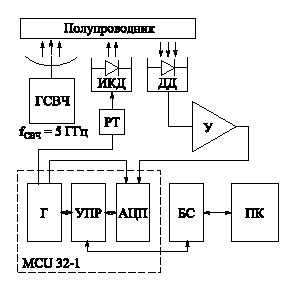
\includegraphics[height=6cm]{pic4_taumetr.eps}
\caption{Схема установки}
\label{pic4_taumetr}
\end{figure}

Генератор СВЧ излучения ГСВЧ создаёт в волноводе стоячую волну. Частота излучения 2.5 ГГц. Через кольцевой зазор в волноводе часть излучения выходит наружу и поглощается в полупроводнике. Величина поглощённой СВЧ мощности пропорциональна концентрации свободных носителей заряда. Данные об интенсивности СВЧ излучения снимаются детекторным СВЧ диодом ДД, усиливаются и отправляются в микроконтроллер.

При освещении полупроводника монохроматическим светом при помощи инфракрасного светодиода ИКД концентрация свободных носителей увеличивается. Длина волны светодиода 1.06 мкм. Прибор снимает изменение концентрации и выводит результат на экран компьютера. Длительность импульса задаётся программно. Запуск измерения производится кнопкой <<Измерить>>, файл с результатами сохраняется в памяти устройства.

Зная, что концентрация избыточных носителей изменяется по закону $\delta n(t) = \Delta n_{0} \exp(-\frac{t}{\tau})$, постоянную $\tau$ можно получить, построив график зависимости $\ln n(t)$. Котангенс угла наклона такого графика будет равен времени жизни.

Влияние поверхностной рекомбинации приводит к искажениям релаксационной кривой в начальной области. Стандарт SEMI MF-1535 рекомендует измерять время жизни по участку от 45\% до 5\% от максимального уровня выходного сигнала. Предел 5\% ограничивает уровень шума.

\subsection{Работа с программой моделирования релаксационной кривой}

Постоянная спада фотопроводимости зависит не только от свойств материала, из которого сделан образец, но и от состояния поверхности. В первом приближении формула (\ref{eq4_pavelka}) даёт близкую оценку величины рекомбинационного времени жизни в объёме полупроводника и скорости поверхностной рекомбинации. Для более точного анализа численными методами решается уравнение непрерывности. Программа расчитывает время жизни в объёме, исходя из данных о концентрации центров рекомбинации, затем строит профиль статического распределения носителей при данном уровне освещения. Затем рассчитывает скорость изменения электропроводности, анализируя изменение концентрации при рекомбинации носителей. После этого расчитывает время жизни по контангенсу угла наклона логарифма кривой спада фотопроводимости и выводит на экран полученное значение эффективного времени жизни с учётом рекомбинации на поверхности. Данные о скорости поверхностной рекомбинации, толщине образца, типе проводимости, концентрации глубоких центров и длине волны засвечивающего светодиода вводятся вручную.

В ходе работы требуется построить зависимость измеряемого времени жизни $\tau_{eff}$ от времени жизни в объёме $\tau$. Для этого на каждом шаге подбирается такая концентрация глубоких уровней $N_{t}$, чтобы $\tau$ менялось от одной микросекунды до 16 миллисекунд, увеличиваясь в два раза на каждом шаге.

\section{Порядок проведения работы и указания по технике безопасности}

\begin{enumerate}
\item Включить компьютер и установку АПК <<Тауметр>>, запустить программу для измерения времени жизни неравновесных носителей заряда.
\item Поместить образец на предметный стол установки, так чтобы образец полностью закрывал кольцевой зазор.
\item Выбрать шаг по времени так, чтобы чтобы релаксационная кривая к концу измерения интервала выходила на насыщение. Время измерения составляет 1000 шагов. Для уменьшения погрешностей проводят серию измерений с одинаковыми параметрами.
\item Выбрать ток засветки так, чтобы уровень инжекции оставался низким. Для этого сравниваются результаты измерения при разных токах лазера, и если значения отличаются более чем на 30\%, ток необходимо уменьшить по меньшей мере вдвое.
\item Расчет эффективного времени жизни производится автоматически. Нулевая точка выбирается как среднее значение последних десяти измерений, максимальная – через два шага после выключения подсветки. В окне «ГОСТ» появляется значение времени, равное моменту времени, в который максимальное значение сигнала уменьшается в 2,7 раз. В окне «ASTM» появляется значение котангенса угла наклона логарифма релаксационной кривой на участке от 45 до 5\% первоначальной интенсивности.
\item Записать результаты измерения в файл для последующей обработки.
\item Запустить программу для расчёта времени жизни.
\item Ввести толщину образца, тип проводимости, длин волны засвечивающего лазера. Сделать предположение о концентрации глубоких уровней $N_{t}$ (величина, обратно пропорциональная времени жизни в объёме полупроводника).
\item Ввести скорость поверхностной рекомбинации, исходя из предположений о пассивации образца.
\item Рассчитать профиль статического распределения, затем запустить расчёт спада фотопроводимости и расчёт времени жизни (ASTM).
\item Результаты внести в таблицу \ref{table4}.
\end{enumerate}

Электрический ток в схеме не превышает 300 мА. При выполении работы действует стандартная техника безопасности при работе с компьютером.

\begin{table}[h!]
\caption{Измерение времени жизни}
\begin{center}
\begin{tabular}{c|c|c}
№ & $\tau$ & $\tau_{eff}$ \\
\hline
& мкс & мкс \\
\hline
\end{tabular}
\end{center}
\label{table4}
\end{table}

\section{Обработка результатов эксперимента}

\begin{enumerate}
\item Из результатов измерения выделить кривую спада фотопроводимости, построить зависимость логарифма избыточной концентрации от времени, выделить линейный участок графика.
\item Меняя концентрацию глубокой примеси в образце при моделировании, построить график зависимости эффективного времени жизни от времени жизни в объёме образца для данной толщины.
\item По полученным данным определить величину времени жизни в объёме полупроводника.
\item Определить погрешность измерения времени жизни неравновесных носителей заряда.
\item Сравнить результаты измерения с формулой (\ref{eq4_pavelka}). Сделать выводы о применимости формулы для образцов данной толщины.
\end{enumerate}

\section{Контрольные вопросы}

\begin{enumerate}
\item Определение времени жизни неравновесных носителей заряда и диффузионной длины неравновесных носителей заряда.
\item Зависимость времени жизни и диффузионной длины неосновных носителей заряда от параметров материала.
\item Центры рекомбинации и прилипания неравновесных носителей заряда.
\item Диффузия и дрейф носителей в полупроводнике.
\item Нестационарные методы измерения времени жизни.
\item Влияние поверхностной рекомбинации на время жизни неравновесных носителей заряда.
\item Соотношение Эйнштейна для определения коэффициента диффузии свободных носителей заряда.
\item Влияние центров прилипания на результаты измерения времени жизни неравновесных носителей заряда.
\item Основные механизмы рекомбинации в полупроводниках.
\item Основные механизмы генерации в полупроводниках.
\end{enumerate}

\section{Литература}
\begin{enumerate}
\item В.В. Батавин, Ю.А. Концевой, Ю.В. Федорович. Измерение параметров полупроводниковых материалов и структур. М.: Радио и связь, 1985 г.
\item Л.П. Павлов. Методы определения основных параметров полупроводниковых материалов. М.: Высшая школа, 1975 г.
\item Шалимова К.В. Физика полупроводников. СПб.: Лань 2011.
\end{enumerate}
\newpage

\anonchapter{Лабораторная работа №5}
\setcounter{chapter}{5}

\begin{center}
Исследование магнетосопротивления полупроводников\\
(4 часа)
\end{center}

\section{Цель работы}
Измерение изменения сопротивления полупроводников в магнитном поле, определение дрейфовой подвижности носителей заряда.

\section{Теоретическая часть}

\subsection{Увеличение электросопротивления полупроводника в магнитном поле}

Эффект магнетосопротивления заключается в изменении электросопротивления обазца при наложении магнитного поля. Причиной возникновения этого эфекта является искривление траектории движения носителей заряда в скрещенных магнитном и электрическом полях.

\begin{figure}[h!]\centering
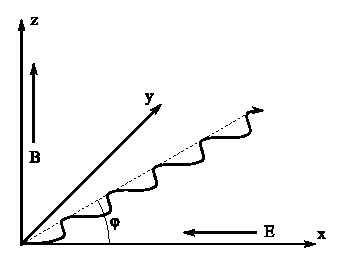
\includegraphics[height=6cm]{pic5_cycloid.eps}
\caption{Траектория электрона в скрещенных электрическом и магнитном полях внутри неограниченного полупроводника}
\label{pic5_cycloid}
\end{figure}

На движущийся заряд в магнитном поле действует сила Лоренца, которая направлена перпендикулярно дрейфовой скорости электронов $\overrightarrow{V}_{d}$ и вектору магнитной индукции $\overrightarrow{B}$. В полупроводнике заряд не может двигаться сколь угодно долго вдоль идеальной траектории, так как испытывает периодические столкновения с дефектами кристаллической решётки. При столкновении теряется энергия и, следовательно, скорость. Таким образом, носители заряда в кристалле двигаются по отрезкам циклоиды (см. рисунок \ref{pic5_cycloid}), при этом среднее направление их движения составляет с направлением поля $\overrightarrow{E}$ некоторый угол $\phi$, называемый углом Холла. Величина угла Холла определяется соотношением между дрейфовой подвижностью носителей $\mu_{d} $ и индукцией магнитного поля:

\begin{equation}
\tg \phi = \mu_{d} B
\end{equation}

Из-за того, что частица движется не по прямой, за время свободного пробега она проходит вдоль поля расстояние меньшее, чем длина свободного пробега $l_{0}$:

\begin{equation}
l_{\text{х}} = l_{0} \cos \phi
\end{equation}

В слабых магнитных полях при малом значении угла Холла

\begin{equation}
l_{\text{х}} = l_{0} \left( 1-\frac{\phi^2}{2} \right) = l_{0} \left( 1-\frac{\mu_{d}^2 B^2}{2} \right)
\end{equation}

Уменьшение пути $l_{\text{х}}$ эквивалентно уменьшению проводимости проводника:

\begin{equation}
\frac{\Delta \rho}{\rho_{0}} = \frac{\rho_{B} - \rho_{0}}{\rho_{0}} = \frac{\sigma_{0} - \sigma_{B}}{\sigma_{B}} = \frac{\l_{0} - \l_{\text{х}}}{\l_{\text{х}}} \approx \frac{\mu_{d}^2 B^2}{2}
\end{equation}

Изменение электросопротивления полупроводника пропорционально квадрату индукции магнитного поля, при этом коэффициент пропорциональности определяется величиной дрейфовой подвижности.

\subsection{Величина магнетосопротивления в ограниченном полупроводнике}

\begin{figure}[h!]\centering
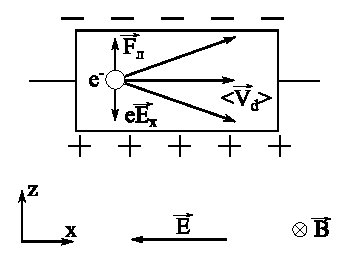
\includegraphics[height=6cm]{pic5_strip.eps}
\caption{Направления движения электронов в ограниченном образце в скрещенных электрическом и магнитном полях}
\label{pic5_strip}
\end{figure}

Рассмотрим полупроводник в виде длинного однородного стержня (рис. \ref{pic5_strip}). Под действием электрического поля $\overrightarrow{E}$ электроны движутся вдоль оси $x$. Со стороны магнитного поля $\overrightarrow{B} \perp \overrightarrow{E}$ на электроны действует сила Лоренца, направленная вдоль оси $z$. Двигаясь под действием силы Лоренца электроны скапливаются на одной из граней, заряжая её отрицательно. На противоположной грани образцется положительный заряд нескомпенсированных ионов примеси. В результате возникает поперечная ЭДС Холла, препятствующая дальнейшему разделению зарядов. Накопление зарядов будет продолжаться до тех пор, пока поле Холла не скомпенсирует отклоняющее действие магнитного поля:

\begin{equation}
e \overrightarrow{E} = -e \left[ \overrightarrow{V}_{d} \times \overrightarrow{B} \right]
\end{equation}

Если бы все электроны в кристалле имели одинаковые скорости, то они двигались бы прямолинейно вдоль оси Ox, так как кулоновская сила создаваемая полем Холла уравновешивается силой Лоренца. Однако в полупроводнике всегда имеет место некоторое распределение электронов по скоростям, обусловленное вероятностным характером рассеяния носителей. Из-за этого электроны, обладающие скоростью ниже средней будут отклоняться к одной грани образца под действием нескомпенсированного поля Холла, а обладающие более высокой скоростью - к другой, под действием нескомпенсированной силы Лоренца. При этом поток электронов в направлении приложенного поля уменьшается, что приводит к уменьшению электропроводности. За счёт того, что продольная скорость уменьшается только для электронов со скоростями, далёкими от средней, увеличение электросопротивления будет менее заментым, нежели в неограниченном образце. В вырожденных полупроводниках и металлах в проводимости участвуют прежде всего электроны, находящиеся вблизи уровня Ферми и обладающие поэтому практически одинаковыми скоростями, поэтому эффект Холла в них будет заметен гораздо меньше, чем в невырожденных полупроводниках.

Более строгий вывод эффекта магнетосопротивления может быть проведён на основе решения кинетического уравнения Больцмана. Решением являются выражения для электропроводности в присутствии магнитного поля

\begin{equation}
\sigma_{B} = e n \left< \frac{\mu}{1 + \mu^2 B^2} \right>
\end{equation}

В области слабых магнитных полей ($\mu B \ll 1$) 

\begin{equation}
\frac{\Delta \rho}{\rho_{0}} = \frac{<\mu^3>}{<\mu>} B^2 = \frac{<\mu^3>}{<\mu>^3}\mu^{2}_{d} B^2 = \frac{<\tau^3>}{<\tau>^3}\mu^{2}_{d} B^2 = C \mu^{2}_{d} B^2
\end{equation}

Величина $C$ характеризует разброс носителей по скоростям и определяется доминирующим механизмом рассеяния.

В сильном магнитном поле ($\mu B \gg 1$) 

\begin{equation}
\frac{\Delta \rho}{\rho_{0}} = \frac{<\mu>}{<\mu^{-1}>} B^2 = \frac{1}{<\mu><\mu^{-1}>} \mu_{d}^2 B^2 = \frac{1}{<\tau><\tau^{-1}>} \mu_{d}^2 B^2
\end{equation}

для ограниченного полупроводника с одним типом носителей, имеющего форму бесконечно длинного стержня, в области слабых магнитных полей ($\mu B \ll 1$) можно считать, что

\begin{equation}
\frac{\Delta \rho}{\rho_{0}} = [C - A^2] \mu^{2}_{d} B^2
\end{equation}
где $C = \frac{\left< \tau^3 \right>}{\left< \tau \right>^3}$, $A = \frac{\left< \tau^2 \right>}{\left< \tau \right>^2}$ - холл-фактор.

\subsection{Диск Корбино}
Удобной моделью неограниченного образца является диск Корбино - образец, выполненный в форме диска с отверстием в центре (рис. \ref{pic5_korbino}). Токовые контакты в таком образце расположены в центральном отверстии и по периферии диска, а магнитное поле направлено перпендикулярно плоскости диска. Линии тока наравлены от цента к краям по радиусу. Под действием магнитного поля линии тока в образце искривляются, но поперечное к электрическому поле Холла не возникает, так как не происходит разделения зарядов в образце.
\chapter{Изучение поглощения света в полупроводниках}

\section{Цель работы}
Целью работы является изучения основных механизмов поглощения света в полупроводниках и освоение методики исследований спектров поглощения света в полупроводниках в видимой и ближней инфракрасной области спектра.

\section{Теоретическая часть}
\subsection{Коэффициент поглощения света}
Если поток фотонов с длиной волны $\lambda$ и интенсивностью $I_{0}(\lambda)$ падает на плоскопараллельный образец толщиной $d$, то можно исследовать интенсивность отражённого от поверхности образца света $I_{R}(\lambda)$ и определить безразмерный коэффициент отражения

\begin{equation}
R(\lambda) = \frac{I_{R}(\lambda)}{I_{0}(\lambda)}
\end{equation}

а также измерить интенсивность прошедшего через образец света $I_{T}(\lambda)$ и определить безразмерный коэффициент пропускания

\begin{equation}
T(\lambda) = \frac{I_{T}(\lambda)}{I_{0}(\lambda)}
\end{equation}

Интенсивность прошедшего через образец света однозначно определяется коэффициентом отражения, поглощением внутри образца и отражением от внутренних граней. Закон Бугера-Ламберта внутри образца, на поверхность которого падает свет выглядит следующим образом:

\begin{equation}
I(x, \lambda) = I_{0}(\lambda) \left[ 1 - R(\lambda) \right] \exp{(- \alpha (\lambda) x )}
\end{equation}
где $\alpha(\lambda)$ - коэффициент поглощения, имеет размерность обратной длины.

Величина $\alpha^{-1}$ определяет толщину кристалла, проходя через которую свет ослабляется в $e$ раз. Это значит, что можно считать величину $\alpha$ вероятностью поглощения фотона на единице длины. Если имеется несколько независимых механизмов поглощения света в кристалле, то полный коэффициент поглощения будет суммой коэффициентов, определяемых каждым механизмом независимо.

\begin{equation}
\alpha(\lambda) = \sum\limits_{i}{\alpha_{i}(\lambda)}
\label{eq6_alphasum}
\end{equation}

Зависимость $\alpha(\lambda)$ называется спектром поглощения для данного вещества.

Практическое использование формулы Бугера-Ламберта приводит к известным проблемам, связанным с невозможностью прямого измерения интенсивности света внутри кристалла на определённой глубине. При измерении интенсивности света, прошедшего через образец толщиной $d$ необходимо учитывать не только поглощение света данным слоем, но также долю отражённого света и сумму всех потоков с учётом многократного отражения. Сумму всех потоков можно представить в виде бесконечной геометрической прогрессии, первый член которой равен $I_{0} (1-R)^2 \exp(-\alpha d)$, а множитель $R^2 \exp(-2 \alpha d)$. Интенсивность света, прошедшего через образец $I_{T}$, таким образом находится как

\begin{equation}
I_{T} = I_{0} \frac{(1-R)^2 \exp(-\alpha d)}{1 - R^2 \exp(-2 \alpha d)}
\end{equation}

Если учесть, что обычно $\alpha d \gg 1$, в знаменателе можно пренебречь вторым членом и считать

\begin{equation}
I_{T} = I_{0} (1-R)^2 \exp(-\alpha d)
\end{equation}

Откуда можно получить коэффициент поглощения на данной длине волны:

\begin{equation}
\alpha = \frac{1}{d} \ln \frac{I_{0} (1-R)^2}{I_{T}}
\label{eq6_alpha_T}
\end{equation}

Если неизвестен коэффициент отражения, то величину $\alpha$ можно определить, сравнивая интенсивность света, прошедшего через два образца из одного материала с одинаковой обработкой поверхностью, но различной толщины. В таком случае для образцов с толщинами $d_{1}$ и $d_{2}$

\begin{equation}
\alpha = \frac{1}{d_{1}-d_{2}} \ln \frac{I_{T1}}{I_{T2}}
\end{equation}

\subsection{Механизмы поглощения света}
Основные механизм поглощения света в полупроводниках определяются возможными типами переходов носителей заряда между зонами, или типами возбуждаемых светом тепловых колебаний решётки кристалла (фононов). Электронные и дырочные механизмы поглощения схематически показаны на рисунке \ref{pic6_transition}.

\begin{figure}[h!]\centering
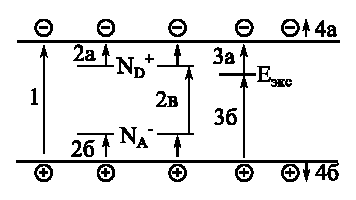
\includegraphics{pic6_transition.eps}
\caption{Схема электронных переходов при различных механизмах поглощения света}
\label{pic6_transition}
\end{figure}

На рисунке обозначены:

\begin{enumerate}
\item Собственное или фундаментальное поглощение света, связанное с переходом электрона из валентной зоны в зону проводимости.
\item примесное поглощение, связанное с переходами электронов с примесного уровня в зону проводимости (2а на рисунке), из валентной зоны на примесный уровень (2б) или между различными примесными центрами (2в).
\item Экситонное поглощение, связанное с возбуждением экситона (переход 3б) или распадом на пару электрон-дырка (3а).
\item Поглощение свободными носителями заряда, сопровождаемое переходом свободных носителей на более высокие энергетические состояния внутри зоны.
\item Фононное поглощение (на рисунке не может быть отражено), связанное с возбуждением в кристалле одного или нескольких фононов - квантов тепловых колебаний решётки.
\end{enumerate}

Рассмотрим форму спектра поглощения для каждого из механизмов по отдельности.

\paragraph{Собственное поглощение}
Рассмотрим поглощение фотона с энергией $E_{\text{ф}} = \hbar \omega$ непрямозонным полупроводником с шириной запрещённой зоны $E_{g} < E_{\text{ф}}$. Пусть зонная структура имеет вид, приведённый на рисунке \ref{pic6_zone}.

\begin{figure}[h!]\centering
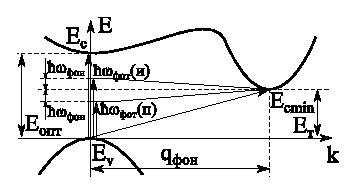
\includegraphics{pic6_zone.eps}
\caption{Схема непрямых переходов электронов при собственном поглощении}
\label{pic6_zone}
\end{figure}

Поглотив фотон, электрон переходит из валентной зоны в зону проводимости. Такие переходы могут происходить как прямым образом (практически без изменения волнового вектора электрона), так и непрямыми (между экстремумами разрешённых зон $E_{c}$ и $E_{v}$). Непрямые переходы требуют значительного изменения волнового вектора электрона.

Можно записать законы сохранения энергии и импульса для прямых переходов

\begin{equation}
E_{1} + \hbar \omega = E_{2}
\end{equation}

\begin{equation}
\overrightarrow{P_{1}} + \hbar \overrightarrow{q} = \overrightarrow{P_{2}}
\end{equation}
где $E_{1}$ и $E_{2}$ - энергии начального и конечного состояния электрона, $\overrightarrow{P_{1}} = \hbar \overrightarrow{k_{1}}$ и $\overrightarrow{P_{2}} = \hbar \overrightarrow{k_{2}}$ - квазиимпульсы электрона в начальном и конечном состоянии. Импульс поглощенного фотона составляет $\hbar \overrightarrow{q}$.Энергия фотона ограничена снизу величиной $\hbar \omega_{min} = E_{g}$, что соответствует длине волны фотона $\lambda_{max} = \frac{\hbar c}{E_{g}}$, где $c$ - скорость света. Если измерять длину волны в микрометрах, а ширину запрещённой зоны в электрон-вольтах, то подставляя известные значения получим удобную формулу:

\begin{equation}
\lambda = \frac{1.24}{E_{g}}
\label{eq6_homega}
\end{equation}

Например, для GaAs ширина запрещённой зоны составляет 1.4 эВ, что соответствует длине волны 0.9 мкм. Значение волнового вектора для фотона с такой энергией составляет:

\begin{equation}
|\overrightarrow{q}| = \frac{2 \pi}{\lambda} \approx 7 \cdot 10^{4}  \text{см}^{-1}
\end{equation}

Волновой вектор электрона можно оценить по формуле

\begin{equation}
|\overrightarrow{k}| = \sqrt{\frac{2 m^{*} k_{0} T}{\hbar^{2}}}
\end{equation}
где $m^{*}$ - эффективная масса электрона, $k_{0}$ - константа Больцмана, $T$ - температура.

При комнатной температуре значение волнового вектора электрона $|\overrightarrow{k}| \approx 10^{7} \text{см}^{-1}$, что значительно больше волнового вектора фотона. Таким образом, в выражении для закона сохранения импульса можно пренебречь импульсом фотона и записать:

\begin{equation}
\overrightarrow{P_{1}} = \overrightarrow{P_{2}}
\end{equation}

или, что то же самое,

\begin{equation}
\overrightarrow{k_{1}} = \overrightarrow{k_{2}}
\end{equation}

Из-за того,что такие переходы идут без изменения волнового вектора, они и названы прямыми.

Спектр поглощения для прямых разрешённых переходов имеет вид

\begin{equation}
\alpha(\hbar \omega) \sim (\hbar \omega - E_{g})^{\frac{1}{2}}
\end{equation}

В свою очередь, для прямых запрещённых переходов

\begin{equation}
\alpha(\hbar \omega) \sim (\hbar \omega - E_{g})^{\frac{3}{2}}
\end{equation}

Суммарный спектр поглощения представляет собой сумму этих двух, а значит при $\hbar \omega \gtrapprox E_{g}$ можно считать, что зависимость коэффициента поглощения определяется только разрешёнными переходами. Если экспериментальные данные спектра вблизи края собственного поглощения построить в координатах $\alpha^2 = f(\hbar \omega)$, то должна получиться прямая линия, точка пересечения которой с осью абсцисс даёт значение ширины запрещённой зоны для прямых переходов (см. рисунок \ref{pic6_direct}).

\begin{figure}[h!]\centering
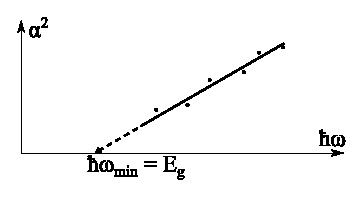
\includegraphics{pic6_direct.eps}
\caption{Представление спектра поглощения для определения ширины запрещённой зоны при прямых переходах}
\label{pic6_direct}
\end{figure}

Для представленного на рисунке \ref{pic6_zone} материала <<оптическая>> ширина запрещённой зоны $E_{\text{опт}}$ оказывается больше, чем минимальная ширина, определяемая как разность между дном зоны проводимости и потолком валентной зоны: $E_{g} = E_{c min} - E_{v}$. Эта величина называется термической шириной запрещённой зоны, так как она определяет термическую активацию электронов в собственном полупроводнике.

В непрямозонном полупроводнике оптические переходы между $E_{c}$ и $E_{v}$ также возможны, но они должны идти при значительном изменении волнового вектора электрона. Так, в Si точки экстремума $E_{v}$ соответствуют центру зоны Бриллюэна, т.е. $|\overrightarrow{k}| = 0$, а для $E_{c}$ находятся вблизи границы в направлении $(100)$, что соответствует $|\overrightarrow{k}| \approx 10^8 \text{см}^{-1}$. Изменение волнового вектора электрона, таким образом, много больше волнового вектора фотона, участвующего в поглощении. Поэтому в процессе поглощения должна использоваться третья частица, волновой вектор которой может достигать подобных значений. Такими частицами в данном случае выступают фононы - кванты тепловых колебаний решётки. Их энергия составляет $\hbar \omega_{\text{фон}} \approx 10^{-2}$ эВ, а волновой вектор $|\overrightarrow{q}| \le 10^{8} \text{см}^{-1}$. Непрямые межзонные оптические переходы могут идти как с поглощением, так и с испусканием фонона. Законы сохранения энергии и импульса для таких переходов будут иметь вид:

\begin{equation}
E_{1} + \hbar \omega_{\text{фот}} \pm \hbar \omega_{\text{фон}} = E_{2}
\end{equation}

\begin{equation}
\overrightarrow{P}_{1} + \hbar \overrightarrow{q}_{\text{фот}} \pm \hbar \overrightarrow{q}_{\text{фон}} = \overrightarrow{P}_{2}
\end{equation}
здесь индексы <<фот>> и <<фон>> относятся к фотону и фонону соответственно. Величиной $\hbar \overrightarrow{q}_{\text{фот}}$ можно пренебречь. Знак минус говорит о процессе испускания фонона, знак плюс - о поглощении.

Спектр поглощения для непрямых переходов описывается следующим образом:

\begin{equation}
\alpha(\hbar \omega_{\text{фот}}) =
C_{1} \frac{\left[ \hbar \omega_{\text{фот}} - (E_{g}-\hbar \omega_{\text{фон}}) \right]^{2}}{\exp \left( \frac{\hbar \omega_{\text{фон}}}{k_{0} T} \right) - 1} +
C_{2} \frac{\left[ \hbar \omega_{\text{фот}} - (E_{g}+\hbar \omega_{\text{фон}}) \right]^{2}}{1 - \exp \left( -\frac{\hbar \omega_{\text{фон}}}{k_{0} T} \right)}
\end{equation}
здесь первый член описывает процессы, связанные с поглощением фононов, второй - с испусканием.

На рисунке \ref{pic6_nondirect} показан спектр поглощения для непрямозонного полупроводника вблизи края собственного поглощения.

\begin{figure}[h!]\centering
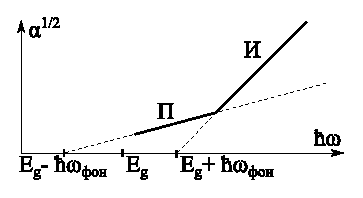
\includegraphics{pic6_nondirect.eps}
\caption{Определение ширины запрещённой зоны и энергии фононов по спектрам поглощения при непрямых переходах}
\label{pic6_nondirect}
\end{figure}

Продолжение участков <<И>> и <<П>> до пересечения с осью абсцисс даст пороговые энергии фотонов для процессов поглощения света, сопровождаемых испусканием и поглощением фонона ($\hbar \omega_{\text{фот}} = E_{g} + \hbar \omega_{\text{фон}}$ и $\hbar \omega_{\text{фот}} = E_{g} - \hbar \omega_{\text{фон}}$) соответственно. Очевидно, значение термической ширины запрещённой зоны $E_{g}$ может быть получено как среднее между этими двумя значениями.

Также в непрямозонном полупроводнике будет наблюдаться поглощение, связанное с прямыми переходами, но оно будет сдвинуто в область более высоких энергий фотонов.

\paragraph{Экситонное поглощение света}
Экситоны - это возбуждённые состояния собственных атомов, которые могут быть представлены в водородоподобной модели как связанная пара электрон-дырка, вращающаяся относительно центра масс. В этой модели эффективная масса экситона $m_{ex}^{-1} = (m_{n}^{-1} + m_{p}^{-1})$. Энергия экситонных состояний равна $E_{ex} = 13.6 \frac{m_{ex}}{m_{0}} \frac{1}{\varepsilon^2} \frac{1}{n^2}$.

Оптические переходы электронов из валентной зоны на экситонные состояния с различными индексами $n$ должны отличаться по энергиям поглощенных фотонов. Так, для уровней 1 и 2:

\begin{equation}
\begin{split}
\hbar \omega_{2} - \hbar \omega_{1} &= \left( E_{g} - E_{ex}(2) \right) - \left( E_{g} - E_{ex}(1) \right) \\
&= E_{ex}(1) -  E_{ex}(2) =  E_{ex}(1) \cdot \left( 1 - \frac{1}{4} \right) \\
&= \frac{3}{4} E_{ex}(1)
\end{split}
\end{equation}

Тогда можно записать:

\begin{equation}
\begin{split}
E_{ex}(1) &= \frac{4}{3} (\hbar \omega_{2} - \hbar \omega_{1}) \\
E_{g} &= \hbar \omega_{1} + E_{ex}(1) = \hbar \omega_{1} + \frac{4}{3} (\hbar \omega_{2} - \hbar \omega_{1})
\end{split}
\end{equation}

На рисунке \ref{pic6_exiton} показан вид экситонного спектра поглощения и диаграмма электронных переходов при оптическом возбуждении экситонов. Экситонные линии спектра расположены вблизи края собственного поглощения. Экситонные состояния заметны лишь в достаточно чистых кристаллах при низких температурах.

\begin{figure}[h!]\centering
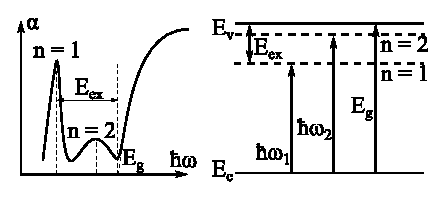
\includegraphics{pic6_exiton.eps}
\caption{Экситонное поглощение света}
\label{pic6_exiton}
\end{figure}

\paragraph{Примесное поглощение света}
Оптическая ионизация примесных центров в полупроводниках связана с переходом электрона из валентной зоны на акцепторный уровень или с донорного уровня в зону проводимости. Энергия фотона, поглощённого при таком переходе, может быть больше или равна энергии ионизации примеси.

Легирующие примеси дают мелкие примесные уровни в запрещённой зоне, и поэтому для их оптической ионизации нужны небольшие энергии: $\hbar \omega \ge 10^{-2}$ эВ, что соответствует далёкой инфракрасной области спектра. Глубокие примесные центры требуют для оптической ионизации гораздо больших энергий. Также возможны переходы с ионизированных примесных состояний в разрешённые зоны - так называемые переходы <<примесь - дальняя зона>>. Так, например, при переходе электрона с акцепторного уровня в зону проводимости, пороговые энергии квантов будут лишь ненамного отличаться от необходимой для собственной ионизации, так как $E_{g} \gg E_{a}-E_{v}$. Таким образом, примесное поглощение, связанное с оптической ионизацией мелких примесей, даёт полосы поглощения в дальней инфракрасной области, а примесное поглощение, связанное с оптической нейтрализацией ионизированных примесных центров, даёт полосы, накладывающиеся на спектр собственного поглощения и создающие <<хвосты>> поглощения при энергиях $\hbar \omega < E_{g}$.

\paragraph{Поглощение света свободными носителями заряда}
Свободные электроны в зоне проводимости, как и свободные дырки в валентной зоне, могут при поглощении света полупроводником переходить внутри своих разрешённых зон в более высокие энергетические состояния. Так как спектр энергий внутри разрешённых зон можно считать непрерывным, то носители могут поглощать фотоны с непрерывно меняющейся энергией, и структурных особенностей для такого спектра наблюдаться не будет. Классическая теория даёт для коэффициента поглощения света свободными носителями заряда следующую зависимость:

\begin{equation}
\alpha(\lambda) = \frac{n e^2 \lambda^2}{8 \pi^2 \tilde{n} c^3 \tau(\overrightarrow{k}) m^{*}}
\label{eq6_nonsel}
\end{equation}
где $\tilde{n}$ - показатель преломления в материале.

Таким образом, коэффициент поглощения растёт по параболическому закону с увеличением длины волны поглощаемых фотонов, и тем больше, чем больше концентрация свободных носителей заряда $n$. Переходы свободных носителей в разрешённых зонах при поглощении фотона оказываются непрямыми, и поэтому для соблюдения законов сохранения импульса и энергии требуют участия ещё одной частицы. Учёт конкретных механизмов рассеяния при поглощении света свободными носителями заряда даёт зависимости $\alpha(\lambda)$ в виде:

\begin{itemize}
\item $\alpha(\lambda) \sim \lambda^{3/2}$ для рассеяния на акустических фононах;
\item $\alpha(\lambda) \sim \lambda^{5/2}$ для рассеяния на оптических фононах;
\item $\alpha(\lambda) \sim \lambda^{7/2}$ для рассеяния на ионах примеси;
\end{itemize}

Анализируя спектр поглощения света в области поглощения свободными носителями можно определить концентрацию свободных носителей и доминирующий механизм рассеяния.

При сложной структуре разрешённых зон возможен не только внутризонный механизм поглощения света, но и поглощение, связанное с переходами между состояниями в различных подзонах в пределах данной разрешённой зоны энергий. Так, например, на рисунке \ref{pic6_subzone} показаны оптические переходы свободных дырок между подзонами тяжёлых (1), лёгких (2) и средних (3) дырок, которые могут происходить в германии и кремнии, а также спектр поглощения при таких переходах. На спектре появляется характерная структура в виде края (1-2) и двух максимумов (2-3 и 1-3). По положению минимума между двумя максимумами можно определить энергию спин-орбитального расщепления $E_{so}$ между подзоной средних дырок и точкой $E_{v max}$ - потолком валентной зоны. Такой характерный спектр поглощения носит название селективного поглощения свободными носителями заряда, в отличие от неселективного, описываемого формулой (\ref{eq6_nonsel}). Этот механизм может наблюдаться также для электронов в зоне проводимости, если зона проводимости имеет сложную структуру в виде частично перекрывающихся подзон энергии.

\begin{figure}[h!]\centering
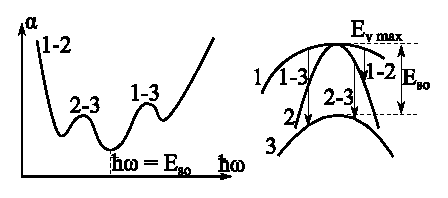
\includegraphics{pic6_subzone.eps}
\caption{Селективное поглощение света свободными дырками}
\label{pic6_subzone}
\end{figure}

\paragraph{Поглощение света тепловыми колебаниями решётки}
Поглощать световую энергию могут не только свободные и связанные электроны и дырки, но и атому кристаллической решётки. При этом в кристалле возникают дополнительные кванты тепловых колебаний решётки, т.е. фононы. Такое поглощение может быть как однофононным (рождение в кристалле одного фонона при поглощении одного фотона), так и многофононным (рождение в кристалле двух и более фононов при поглощении одного фотона). В силу законов сохранения при однофононным поглощении света могут возникать только поперечные оптические фононы (т.к. фотон - квант поперечного электромагнитного поля). Такое поглощение имеет специфический остро резонансный характер, так как в каждом кристалле может с некоторой максимальной вероятностью возникать только вполне определённый тип поперечных оптических фононов. Коэффициент поглощения света при однофононном поглощении весьма велик у кристаллов с большой долей ионной связи. Так как кристаллы сильно отражают свет в той области, где велико его поглощение, то в спектре отражения ионных кристаллов наблюдается резонансный пик отражения света, связанный с однофононным поглощением. Это отражение получило название <<явления остаточных лучей>> и использовалось в спектроскопии для монохроматизации света в ИК-области спектра.

В полупроводниках с большой долей ковалентных связей наблюдается преимущественно многофононное поглощение света решёткой кристалла. При этом поглощённый фотон порождает в кристалле вполне определённый набор комбинаций фононов. Например, $LO + 2 TA$ - продольный оптический и два поперечных акустических фонона. Такие наиболее вероятные комбинации фононов дают острые пики в спектре поглощения света в далёкой ИК-области. Характеристические спектры решёточного многофононного поглощения накладывается обычно на спектр поглощения свободными носителями заряда, который также даёт существенный вклад в далёкой ИК-области спектра.

\paragraph{Общий спектр поглощения света}
В силу соотношения (\ref{eq6_alphasum}), общий спектр поглощения для данного образца может быть получен как сумма спектров каждого отдельного механизма. Общая картинка спектра в широком диапазоне длин волн может иметь вид, представленный на рисунке \ref{pic6_spectrum}.

\begin{figure}[h!]\centering
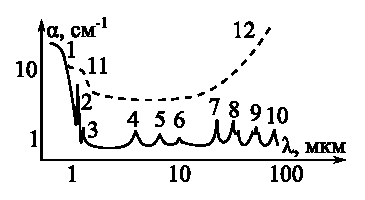
\includegraphics{pic6_spectrum.eps}
\caption{Общий вид спектра поглощения света в полупроводниках. Сплошная линия - слаболегированный, пунктирная - сильнолегированный материал. 1 - край собственного поглощения; 2,3 - экситоны и экситонно-примесные комплексы; 4,5,6 - примесное поглощение; 7,8,9,10 - многофононное поглощение; 11 - сдвиг края собственного поглощения в сильнолегированном образце; 12 - неселективное поглощение свободными носителями.}
\label{pic6_spectrum}
\end{figure}

В коротковолновой части спектра лежит край собственного поглощения, вблизи которого может наблюдаться характерная структура экситонного спектра. В области более длинных волн за краем собственного поглощения могут наблюдаться примесные полосы поглощения, соответствующие глубоким примесным центрам. Поглощение свободными носителями заряда монотонно растёт с длиной волны в ИК-области спектра. На него накладывается характерная структура многофононного решёточного поглощения света. Вид спектра поглощения кристалла существенно зависит от концентрации примесей в полупроводнике. При возрастании концентрации легирующей примеси растёт поглощение на свободных носителях заряда (в длинноволновой области), пропадает экситонная структура вблизи края собственного поглощения, сам край собственного поглощения может сдвигаться в коротковолновую область за счёт эффекта Бурштейна-Мосса.

\section{Методика измерений и описание установки}
Для определения спектра поглощения $\alpha(\lambda)$ требуется знать коэффициент пропускания $T(\lambda)$, толщину образца $d$ и коэффициент отражения $R(\lambda)$. В данной работе можно считать коэффициент отражения равным нулю, а коэффициент поглощения таков, что $\alpha d < 1$, что позволяет воспользоваться достаточно простой формулой (\ref{eq6_alpha_T}).

Блок-схема установки приведена на рисунке \ref{pic6_scheme}.

\begin{figure}[h!]\centering
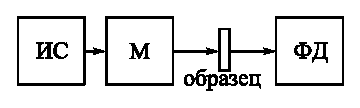
\includegraphics{pic6_scheme.eps}
\caption{Блок-схема измерительной установки. Здесь ИС - источник света с фокусирующей системой, М - монохроматор, ФД - фотодатчик с регистрирующим устройством.}
\label{pic6_scheme}
\end{figure}

В ходе работы из непрерывного спектра, даваемого источником, необходимо выделять отдельные длины волн. Для этого используется универсальный монохроматор УМ-2. В качестве источника сплошного спектра принимается отверстие в полости с температурой $T$, которую имитирует лампа накаливания с температурой нити 3000 К. Разложение непрерывного спектра производится при помощи призмы, при этом длина волны, подаваемая на выход монохроматора, определяется углом поворота призмы. Угол может плавно меняться вращением барабана. При работе с монохроматорами такого рода необходима градуировка, которая позволит поставить в соответствие углу поворота призмы длину волны, получаемую на выходе. Для градуировки используется ртутная лампа, в спектре которой наблюдаются яркие полосы. Длины волн некоторых линий спектра ртути приведены в таблице \ref{table6_Hg}.

\begin{table}[h]
\caption{Длины волн некоторых линий спектра ртути}
\begin{center}
\begin{tabular}{c|c|c}
Цвет & Длина волны, нм & Угол поворота барабана \\
\hline
Глубокий красный & 730 & \\
Красный & 623 & \\
Красный & 619 & \\
Оранжевый & 607 & \\
Желтый & 579 & \\
Желтый & 576 & \\
Зелёный & 546 & \\
Голубой & 491 & \\
Синий & 435 & \\
Фиолетовый & 408 & \\
Фиолетовый & 404 & \\
\hline
\end{tabular}
\end{center}
\label{table6_Hg}
\end{table}

Образец для измерения спектра поглощения должен иметь вид тонкой плоскопараллельной пластины с отполированными поверхностями. Держатель для образца имеет вид шторки с двумя прорезями, в одну из которых вставляется образец. Коэффициент пропускания на данной длине волны определяется как отношение интенсивности света прошедшего через образец к интенсивности света, прошедшего через незакрытую прорезь в шторке: $T(\lambda) = I_{\text{обр}}(\lambda)/I_{\text{0}}(\lambda)$.

Интенсивность выходного сигнала определяется как величина, пропорциональная выходному сигналу фотодетектора $U$. Выходной сигнал снимается универсальным вольтметром В7-16А.

\section{Порядок проведения работы и указания по технике безопасности}

\begin{enumerate}
\item Произвести градуировку монохроматора, для чего 
	\begin{enumerate}
	\item установить на рельс ртутную лампу, включить блок питания и дать ей прогреться;
	\item установить необходимый размер входной щели и фокусировку линзы для визуального различения жёлтого дуплета ртути;
	\item выводить поочерёдно спектральные линии ртути и фиксировать в таблице \ref{table6_Hg} показания барабана поворотного устройства призмы монохроматора.
	\end{enumerate}
\item Произвести измерение пропускания $T(\lambda)$ образца, для чего
	\begin{enumerate}
	\item установить на рельс лампу накаливания и включить блок питания, сфокусировать световое пятно на входной щели монохроматора;
	\item установить шторку с прорезью перед выходной щелью;
	\item установить фотодетектор за выводной щелью;
	\item плавно вращая барабан монохроматора, фиксировать различие в выходном сигнале фотодетектора при пропускании света через прорезь без образца и через образец;
	\item Внести результаты измерений в таблицу \ref{table6_data}
	\end{enumerate}
\item Построить спектр поглощения образца в осях $\alpha^2 = f(\hbar \omega)$ и $\alpha^{1/2} = f(\hbar \omega)$. Сравнивая графики, сделать выводы о прямозонности материала.
\end{enumerate}

\begin{table}[h]
\renewcommand{\arraystretch}{1.8} %% increase table row spacing
\caption{Спектр поглощения образца}
\begin{center}
\begin{tabular}{c*{5}{|c}}
Угол & $\lambda$ & $U_{0}$ & $U_{\text{обр}}$ & $T(\lambda)$ & $\alpha$ \\
\hline
 & нм & мВ & мВ &  & $\text{см}^{-1}$ \\
\hline
\end{tabular}
\end{center}
\label{table6_data}
\end{table}

Соблюдается стандартная техника безопасности при обслуживании высокоточных (до 3 А) источников. В ходе работы используются яркие лампы, на которые не рекомендуется смотреть невооружённым глазом.

\section{Обработка результатов эксперимента}
\begin{enumerate}
\item По линейной интерполяции данных таблицы \ref{table6_Hg} определяется формула пересчёта угла поворота призмы в длину волны в виде $y = a x + b$, где $y$ - длина волны, $x$ - угол.
\item По полученной формуле значения угла пересчитываются в энергию фотона с учётом соотношения (\ref{eq6_homega}).
\item Для прямозонного материала ширина запрещённой зоны определяется по линейной экстраполяции коэффициента поглощения на ось абсцисс в координатах $\alpha^2 = f(\hbar \omega)$, как это показано на рисунке \ref{pic6_direct}.
\item Для непрямозонного материала ширина запрещённой зоны определяется по экстраполяциям линейных участков, как это показано на рисунке \ref{pic6_nondirect}.
\item Исходя из полученной ширины запрещённой зоны делается вывод о том, какой материал был использован в данной работе.
\end{enumerate}

\section{Контрольные вопросы}
\begin{enumerate}
\item Понятие коэффициента поглощения. Размерность и порядок этой величины для полупроводников.
\item Как связаны величины $T$, $R$ и $\alpha$.
\item Основные механизмы поглощения света в полупроводниках.
\item Общий вид спектра поглощения и влияние на него легирующих примесей.
\item Вид спектра собственного поглощения и методы его анализа для прямых и непрямых переходов.
\item Определение ширины запрещённой зоны по краю собственного поглощения.
\item Факторы, влияющие на положение края собственного поглощения.
\item Экситонный спектр поглощения.
\item Почему экситонный спектр не наблюдается в поглощении при комнатной температуре, а также при высокой степени легирования образца?
\item Примесное поглощение света в полупроводниках.
\item Поглощение света тепловыми колебаниями решётки.
\item Механизмы поглощения света свободными носителями заряда.
\item Учёт влияния многократного отражения на измерение коэффициента поглощения.
\item Принцип работы монохроматора.
\end{enumerate}

\section{Литература}
\begin{enumerate}
\item П.С. Киреев. Физика полупроводников. СПб.: Лань, 2011 г.
\item В.В. Батавин, Ю.А. Концевой, Ю.В. Федорович. Измерение параметров полупроводниковых материалов и структур. М.: Радио и связь, 1985 г.
\item В.Н. Мартынов, Г.И. Кольцов. Полупроводниковая оптоэлектроника. М.: МИСИС, 1999 г.
\item В.В. Горбачев, Л.Г. Спицина. Физика полупроводников и металлов. М.: Высшая школа, 1986 г.
\end{enumerate}
\chapter{Изучение собственной и примесной фотопроводимости полупроводников}

\section{Цель работы}
Измерение спектра собственной и примесной фотопроводимости полупроводника. Определение ширины запрещённой зоны и энергии ионизации примеси. Исследование влияния поверхностной рекомбинации на форму спектра фотопроводимости.

\section{Теоретическая часть}
\subsection{Фотопроводимость}
При освещении полупроводника светом с достаточной энергией фотонов может возникнуть внутренний фотоэлектрический эффект, или иначе - фотопроводимость. Причиной появления  избыточной фотопроводимости может являться как увеличение концентрации свободных носителей заряда в результате оптической генерации, так и повышение подвижности в результате перехода носителей из подзоны с более тяжёлыми носителями в подзону более лёгких. Во втором случае общее количество носителей остаётся неизменным, но за счёт увеличения подвижности удельное электросопротивление материала падает. Этот эффект может наблюдаться при низких температурах.

В дальнейшем будем считать подвижность носителей постоянной, и рассматривать исключительно повышение проводимости материала за счёт изменения концентрации носителей. Это увеличение может быть связано с процессом фотоионизации атомов основного вещества или примеси, то есть, с собственным и примесным поглощением света в полупроводнике.

\subsection{Собственная и примесная фотопроводимость}
Оптическое излучение на собственной полосе поглощения полупроводника переводит валентные электроны в зону проводимости, то есть, приводит к генерации избыточных электронов в зоне проводимости и дырок в валентной зоне в равных соотношениях, если отсутствует захват преимущественный захват электронов или дырок ловушками.
Изменение проводимости полупроводника под действием освещения собственным светом описывается избыточной фотопроводимостью $\Delta \sigma$, определяемый как разница между величинами удельной электропроводности в освещённом и затемнённом состояниях:

\begin{equation}
\Delta \sigma = \sigma - \sigma_{\text{т}} = e (\mu_{n} \Delta n + \mu_{p} \Delta p).
\end{equation}

В широкозонных полупроводниках при комнатной температуре собственная концентрация носителей очень мала, и поэтому избыточная фотопроводимости может на порядки превышать темновую. В узкозонных ($E_{g} \le 1 \text{эВ}$) наоборот концентрация избыточных носителей мала по сравнению с собственной, и поэтому практически всегда реализуется условие малого уровня инжекции.

Длинноволновая граница собственной фотопроводимости совпадает с краем собственного поглощения и для узкозонных полупроводников лежит в инфракрасной области спектра. Для широкозонных полупроводников она может лежать в синей или даже ультрафиолетовой области. Связь между пороговой длиной волны и шириной запрещённой зоны для случая собственной фотопроводимости определяется известным соотношением:

\begin{equation}
\lambda_{\text{гр}} = \frac{h c}{E_{g}} = \frac{1240}{E_{g}}
\end{equation}
где $E_{g}$ выражается в электрон-вольтах, а $\lambda_{\text{гр}}$ - в нанометрах.

При фотоионизации примесей возрастает концентрация электронов в зоне проводимости или дырок в валентной зоне. При этом происходят переходы между уровнями примеси внутри запрещённой зоны и разрешёнными зонами. Такая фотопроводимости называется примесной.

\subsection{Спектральная зависимость фотопроводимости}
В общем случае отношение фотопроводимости к интенсивности падающего света - так называемая фоточувствительность - зависит от длины волны. Для анализа спектра фотопроводимости рассмотрим уравнение непрерывности:

\begin{equation}
\frac{\partial (\Delta n)}{\partial t} = \frac{1}{e} div \overrightarrow{j_{n}} + G_{n} - \frac{\Delta n}{\tau_{n}}
\end{equation}
для электронов.

Если мы рассмотрим полупроводник в отсутствии электрического тока, то в стационарном состоянии уравнение имеет решение:

\begin{equation}
\Delta n = G_{n} \tau_{n}
\end{equation}

А для фотопроводимости можно записать

\begin{equation}
\Delta \sigma = q (\mu_{n} G_{n} \tau_{n} + \mu_{p} G_{p} \tau_{p})
\end{equation}

Так как величина $G_{n}$ зависит от интенсивности падающего излучения $I$ и коэффициента поглощения на данной длине волны $\alpha(\lambda)$, то и фотопроводимость будет определяться этими величинами. Для случая малого уровня инжекции зависимость времени жизни от концентрации носителей можно считать пренебрежимо малой.

Пусть на полупроводник толщиной $d$ падает свет с длиной волны $\lambda$, коэффициент поглощения на данной длине волны составляет $\alpha$. Тогда если образец достаточно тонкий, то есть, $\alpha d \ll 1$, то излучение равномерно поглощается по всему объёму образца, и избыточные носители заряда генерируются равномерно. Если $I$ - интенсивность падающего излучения, то энергия, поглощаемая в единице объёма образце будет равна $\alpha I$, а значит количество электрон-дырочных пар, генерируемых в единице объёма за единицу времени, равно $\eta \alpha I / h \nu$. Здесь $\eta$ - внутренний квантовый выход, то есть, вероятность того, что поглощённый фотон генерирует пару электрон-дырка.
Таким образом, скорость оптической генерации равна

\begin{equation}
G_{n} = \eta_{n} \frac{\alpha I}{h \nu} = \eta_{n} \alpha Q
\end{equation}
где $Q = I / h \nu$  - поток фотонов.

С учётом этого, можно записать спектральную зависимость фотопроводимости полупроводника:

\begin{equation}
\Delta \sigma = q (\eta_{n} \tau_{n} \mu_{n} + \eta_{p} \tau_{p} \mu_{p}) \alpha Q
\end{equation}

\subsection{Спектральная характеристика собственной фотопроводимости}
При равномерной генерации носителей и при отсутствии поверхностной рекомбинации, спектр собственной фотопроводимости определяется спектральной зависимостью коэффициента собственного поглощения. Например, для разрешённых прямых переходов коэффициент поглощения определяется формулой

\begin{equation}
\alpha(h \nu) = \frac{e^2 \left( 2 \frac{m_{n} m_{p}}{m_{n} + m_{p}} \right)^{3/2}}{\tilde{n} c h^2 m_{n}} \cdot (h \nu - E_{g})^{1/2}
\end{equation}

Собственная фотопроводимость при прямых переходах резко возрастает при энергии фотона $h \nu \ge E_{g}$, и при дальнейшем увеличении энергии практически не меняется.

Рассмотрим случай неравномерного поглощения, когда толщиной образца уже нельзя пренебречь. В таком случае

\begin{equation}
G_{y} = \frac{\alpha I_{0} (1-R)}{h \nu} \exp(-\alpha y)
\end{equation}

Будем считать, что толщина образца такова, что излучение практически не достигает дальней стенки образца. Тогда с ростом энергии фотона в основной полосе коэффициент поглощения увеличивается, а значит скорость генерации резко уменьшается по мере прохождения излучения вглубь образца. Из-за этого спектральная зависимость фотопроводимости с увеличением энергии фотонов проходит через максимум, а затем быстро уменьшается.

Учёт влияния поверхностной рекомбинации приводит к уменьшению концентрации вблизи поверхности образца. Если предполагать, что оптическое поглощение происходит равномерно по всему объёму, то единственным изменением, связанным с рекомбинацией на поверхности, будет замена величины $\tau$ на некоторое эффективное время жизни $\tau_{eff}$, зависящее как от времени жизни в объёме $\tau_{v}$, так и поверхностного времени жизни $\tau_{s} = \frac{d}{2 S} + \frac{d^2}{\pi^2 D}$, где $D$ - коэффициент диффузии, а $S$ - скорость поверхностной рекомбинации:

\begin{equation}
\frac{1}{\tau_{eff}} = \frac{1}{\tau_{v}} + \frac{1}{\tau_{s}}
\end{equation}

Это значит, что фотопроводимость при учёте поверхностной рекомбинации окажется в $\frac{\tau_{v}}{\tau_{eff}}$ раз меньше, чем было бы при $S = 0$. При этом поверхностная рекомбинация влияет не только на стационарное значение, но и на вид спектра фотопроводимости. Так, при измерении спектра фотопроводимости в основной полосе поглощения, где коэффициент поглощения сильно возрастает, сказываются два конкурирующих процесса: за счёт увеличения коэффициента поглощения увеличивается величина фотопроводимости, в то же время доля избыточной концентрации, генерируемая вблизи поверхности возрастает, а именно там поверхностные эффекты влияют наиболее заметно. Эти процессы приводят к тому, что в спектральной зависимости фотопроводимости будет наблюдаться максимум фотопроводимости вблизи края собственного поглощения, и чем больше величина $S$, тем сильнее будет выражен этот максимум. Структурные особенности спектра фотопроводимости с учётом влияния поверхностной рекомбинации приведёт на рисунке \ref{pic7_SR}, на нём же приведена кривая спектра поглощения (штрихпунктирная линия). Чтобы учесть этот эффект за длинноволновую границу собственной фотопроводимости принимается длина волны $\lambda_{\frac{1}{2}}$ на длинноволновом спаде спектральной характеристики, при которой фотопроводимость уменьшается в два раза по сравнению с максимальной.

\begin{figure}[h!]\centering
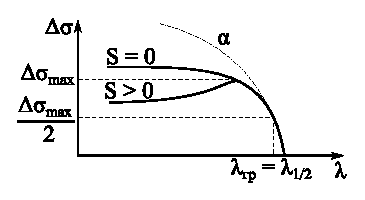
\includegraphics{pic7_SR.eps}
\caption{Спектр собственной фотопроводимости при отсутствии $(S = 0)$ и наличии $(S > 0)$ поверхностной рекомбинации}
\label{pic7_SR}
\end{figure}

\subsection{Спектральная характеристика примесной фотопроводимости}
В примесном кристалле оптические переходы электронов между локальными уровнями примесей (или других нарушений идеальности кристаллического поля) и главными энергетическими зонами приводят к появлению примесного поглощения и примесной фотопроводимости. Так как энергия ионизации мелких примесей лежит вблизи основных зон, то примесная фотопроводимость занимает на спектре область длин волн вблизи края собственной проводимости, а также имеет несколько полос в длинноволновой области, в зависимости от того, какой электронный переход примесь-зона имеет место.

Спектр примесной фотопроводимости достаточно хорошо совпадает со спектром примесного поглощения. Рассмотрим основные оптические переходы в полупроводнике, приводящие к фотопроводимости. Если мелкий уровень нейтрален, то под действием кванта излучения $h \nu \ge E_{i}$, где $E_{i}$  - энергия ионизации примеси, электрон из валентной зоны перейдёт на акцепторный уровень или с донорного уровня перейдёт в зону проводимости. Такие переходы сопровождаются поглощением в области длин волн между $\lambda_{i}$ и $\lambda_{\text{гр}}$. Здесь поглощение растёт с уменьшением длины волны и резко обрывается при $\lambda = \lambda_{\text{i}}$.

Если мелкий уровень ионизован, в области $\lambda \le \lambda_{\text{гр}}$ возникают полосы поглощения, связанные с переходами электронов из валентной зоны на уровень ионизованных доноров или с уровней ионизованных акцепторов в зону проводимости. На рисунке \ref{pic7_transition} показаны обе группы переходов: 1 и 2 - переходы с уровня ионизованного акцептора в зону проводимости, 3 и 4 - переход из валентной зоны на ионизованный донор. Энергия этих переходов близка к ширине запрещённой зоне, и поэтому полосы поглощения, связанные с этими переходами, образуют в длинноволновой части края собственного поглощения ступеньку. Цифрами 5 и 6 обозначены переходы электронов между мелким уровнем и ближней зоной. Энергия таких переходов много меньше ширины запрещённой зоны. Эти переходы заметны только при достаточно глубоком охлаждении полупроводника.

\begin{figure}[h!]\centering
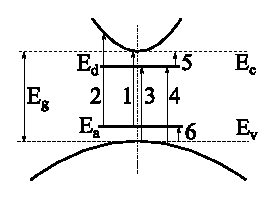
\includegraphics{pic7_transition.eps}
\caption{Схема возможных переходов в примесном кристалле}
\label{pic7_transition}
\end{figure}

В случае переходов 1, 2 и 5 в переносе заряда будут участвовать свободные электроны. Для переходов 3, 4 и 6 такими носителями являются дырки.

Рассмотрим схему оптического поглощения, связанного с переходами электронов с ионизованных акцепторов в зону проводимости. Интервал энергий фотона, соответствующий поглощению, определяется величиной вектора $\overrightarrow{k}_{a}$ волновой функции электрона на акцепторе. Величины волнового вектора, для которых волновые функции будут значительны, находятся в пределах обратного радиуса боровской орбиты акцепторного состояния. Поэтому область энергий с достаточно большим поглощением будет определяться границами:

\begin{equation}
E_{g} - E_{a} < h \nu < E_{g} - E_{a} + E_{c}(\overrightarrow{k}_{a})
\end{equation}

На рисунке \ref{pic7_transition} акцепторный уровень изображён в виде горизонтальной линии, длина которой в k-пространстве равна $|\overrightarrow{k}_{a}|$. Количественно спектр поглощения, связанный с переходами $E_{a} \rightarrow E_{c}$ представляется формулой:

\begin{equation}
\alpha = \frac{A N_{a}}{1+\exp \left[ \frac{E_{a} - F}{k T} \right]} \cdot \frac{h \nu - E_{g} + E_{A}}{h \nu}
\end{equation}
где $A$ - постоянный множитель, не зависящий от частоты, $N_{a}$ - концентрация акцепторных состояний, $F$ - уровень Ферми.

Спектр примесного поглощения имеет ту же зависимость от частоты, что и поглощение, связанное с разрешёнными прямыми межзонными переходами. Только величины поглощения значительно меньше основного и предшествуют основному по шкале энергий фотонов. Отличие также состоит в том, что поглощение зависит от концентрации акцепторных примесей $N_{a}$ и температуры.

Поглощение, вызванное переходами электронов с акцепторного уровня в зону проводимости, будет проявляться в виде широкой полосы и перекрываться с полосой собственного поглощения. Спектр примесной фотопроводимости в этом случае будет представлять собой ступеньку в длинноволновой части спектра (см. рисунок \ref{pic7_spectrum}). Энергия ионизации примеси определяется по положению точки на длинноволновом спаде, где примесная фотопроводимости составляет половину от максимального значения в примесной области поглощения. Значение энергии ионизации, определённое таким образом из спектра поглощения, находится в хорошем согласии со значениями $E_{i}$, полученными другими методами.

\begin{figure}[h!]\centering
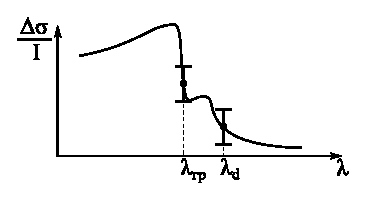
\includegraphics{pic7_spectrum.eps}
\caption{Спектры фотопроводимости примесного полупроводника при поглощении акцепторная примесь - зона проводимости}
\label{pic7_spectrum}
\end{figure}

\section{Методика измерений и описание установки}
Для определения спектра фотопроводимости необходимо знать зависимость фотопроводимости образца и интенсивности источника от длины волны. В данной работе в качестве образца используется фоторезистор, сопротивление которого измеряется при помощи универсального вольтметра В7-138. Чувствительность детектора очень велика, поэтому при измерении его необходимо затемнять.

Измерение спектра фоточувствительности можно проводить в относительных единицах, что позволит избежать трудоёмких измерений абсолютного значения интенсивности света. Для этого достаточно знать спектр относительной интенсивности данного источника для данной длины волны. В работе в качестве источника используется мощная галогенная лампа накаливания с температурой нити 3000 К. Её спектр совпадает со спектром абсолютно чёрного тела. Мощность излучения абсолютно чёрного тела на единицу площади излучающей поверхности в единичном интервале частот может быть определена по формуле Планка:

\begin{equation}
R(\lambda, T) = \frac{2 \pi h c^2}{\lambda^5} \frac{1}{\exp \left( \frac{h c}{\lambda k T} \right) - 1}
\label{eq7_intencity}
\end{equation}
размерность мощности в СИ: $\frac{\text{Дж}}{\text{с} \cdot \text{м}^2 \cdot \text{Гц}}$

Для выделения определённой длины волны из сплошного спектра источника используется монохроматор МДР-3. Разложение света производится при помощи дифракционной решётки, которая может вращаться вокруг своей оси.

\section{Порядок проведения работы и указания по технике безопасности}

\begin{enumerate}
\item Установить держатель с образцом за выходным отверстием монохроматора, установить лампу перед входным отверстием монохроматора.
\item Сфокусировать изображение лампы при помощи системы линз.
\item Установив регулировочную ручку при выходном отверстии образца в положение <<Закрыто>> записать значение сопротивления образца в темноте ($R_{0}$).
\item Меняя длину волны на выходе монохроматора записывать сопротивление образца. Включение двигателя, поворачивающего дифракционную решётку, производится тумблером на лицевой панели монохроматора.
\item После окончания измерений снова измерить темновое сопротивление образца.
\item Внести данные в таблицу \ref{table7_data}
\end{enumerate}

\begin{table}[h!]
\caption{Спектр фотопроводимости образца}
\begin{center}
\begin{tabular}{c|c|c|c|c}
$\lambda$ & $R(\lambda)$ & $\sigma(\lambda)$ & $I(\lambda)$ & $\sigma(\lambda) / I(\lambda)$ \\
\hline
нм & Ом & Сим & отн.ед. & отн.ед. \\
\hline
\end{tabular}
\end{center}
\label{table7_data}
\end{table}

В ходе работы используются яркие лампы, на которые не рекомендуется смотреть невооружённым глазом.

\section{Обработка результатов эксперимента}

\begin{enumerate}
\item Для каждого значения сопротивления $R(\lambda)$ рассчитать величину фотопроводимости $\sigma(\lambda)$ с учётом темновой проводимости.
\item Для каждой длины волны рассчитать относительную интенсивность источника, используя формулу \ref{eq7_intencity} и считая, что интенсивность прямо пропорциональна мощности излучения.
\item Рассчитать фоточувствительность как отношение фотопроводимости к интенсивности света.
\item Построить спектр фоточувствительности от энергии фотонов.
\item По полувысоте края проводимости определить ширину запрещённой зоны полупроводника. По полувысоте примесной ступеньки определить энергию ионизации примеси.
\end{enumerate}

\section{Контрольные вопросы}

\begin{enumerate}
\item Понятие фотопроводимости полупроводника.
\item Основные механизмы поглощения света, которые приводят к появлению фотопроводимости.
\item Собственная и примесная фотопроводимость.
\item Длинноволновая граница фотопроводимости.
\item Скорость оптической генерации электронно-дырочных пар в случае равномерного поглощения оптического излучения по толщине образца.
\item Определение спектра фотопроводимости полупроводников. Чем определяется форма спектра?
\item Влияние скорости поверхностной рекомбинации на форму спектра фотопроводимости.
\item Чем определяется форма края фотопроводимости.
\item Уравнение непрерывности при освещении полупроводника монохроматическим светом.
\item Как соотношение между временем жизни в объёме и на поверхности влияет на форму спектра фотопроводимости?
\end{enumerate}

\section{Литература}
\begin{enumerate}
\item П.С. Киреев. Физика полупроводников. СПб.: Лань, 2011 г.
\item В.В. Батавин, Ю.А. Концевой, Ю.В. Федорович. Измерение параметров полупроводниковых материалов и структур. М.: Радио и связь, 1985 г.
\item В.Н. Мартынов, Г.И. Кольцов. Полупроводниковая оптоэлектроника. М.: МИСИС, 1999 г.
\item В.В. Горбачев, Л.Г. Спицина. Физика полупроводников и металлов. М.: Высшая школа, 1986 г.
\end{enumerate}
\end{document}